\documentclass[a4paper, 11pt]{article}
\usepackage{comment} 
\usepackage{fullpage}
\usepackage{amsmath} 
\usepackage{amssymb} 
\usepackage{mathtools}
\usepackage{siunitx}
\usepackage{xfrac}
\usepackage{icomma}
\usepackage[section,below]{placeins}
\usepackage[labelfont=bf,font=small,width=0.9\textwidth]{caption}
\usepackage{subcaption}
\usepackage{graphicx}
\usepackage{grffile}
\usepackage{float}
\floatplacement{figure}{htbp}
\floatplacement{table}{htbp}
\usepackage{booktabs}
\usepackage{hyperref}
\usepackage{pdfpages}
\sisetup{separate-uncertainty=true}

\begin{document}
\noindent
\centerline{\small{\textsc{Michigan State University}}} \\
\large{\textbf{CMSE 823 – Numerical Linear Algebra \hfill Spring 2020 \\
Homework 6}} \\
Alexander Harnisch \\
\noindent\makebox[\linewidth]{\rule{\textwidth}{0.4pt}}

\section*{1.}
See the following two handwritten pages.
\FloatBarrier
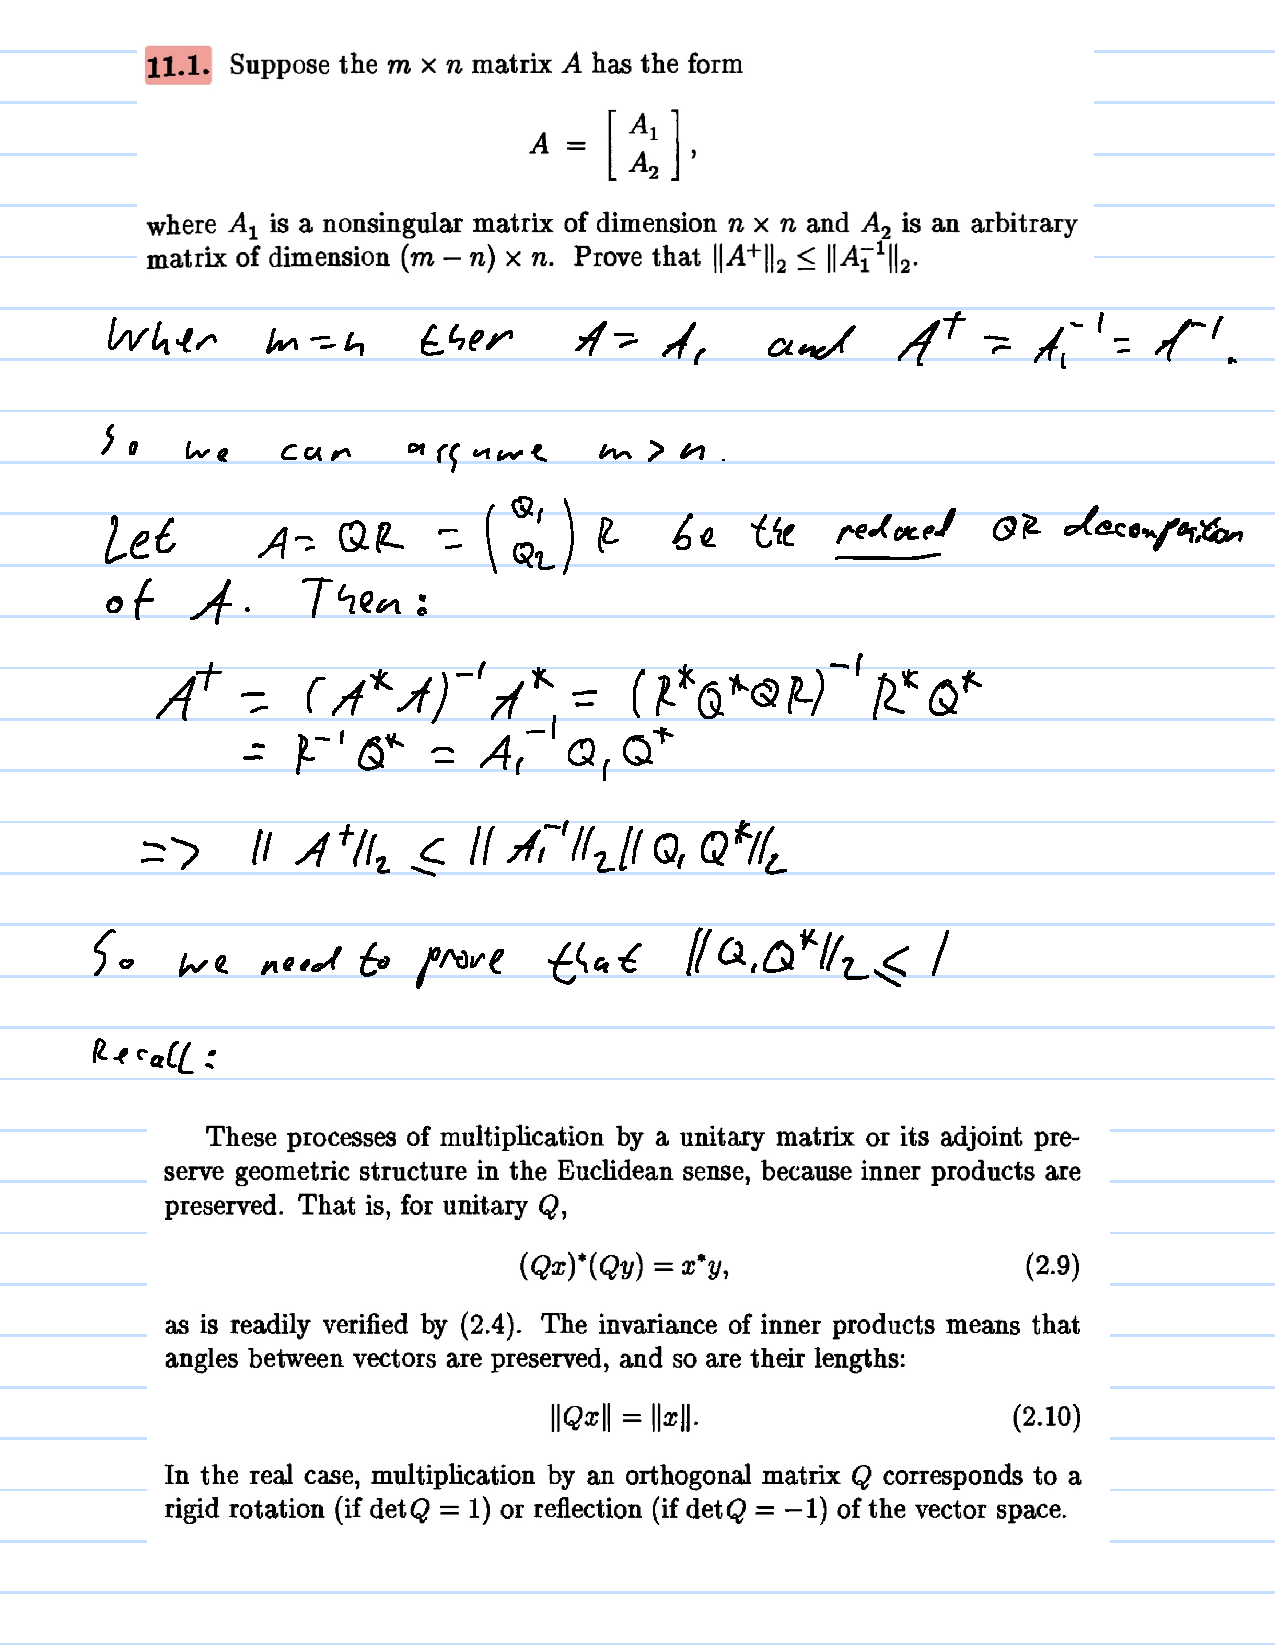
\includepdf{../1/1_1.pdf}
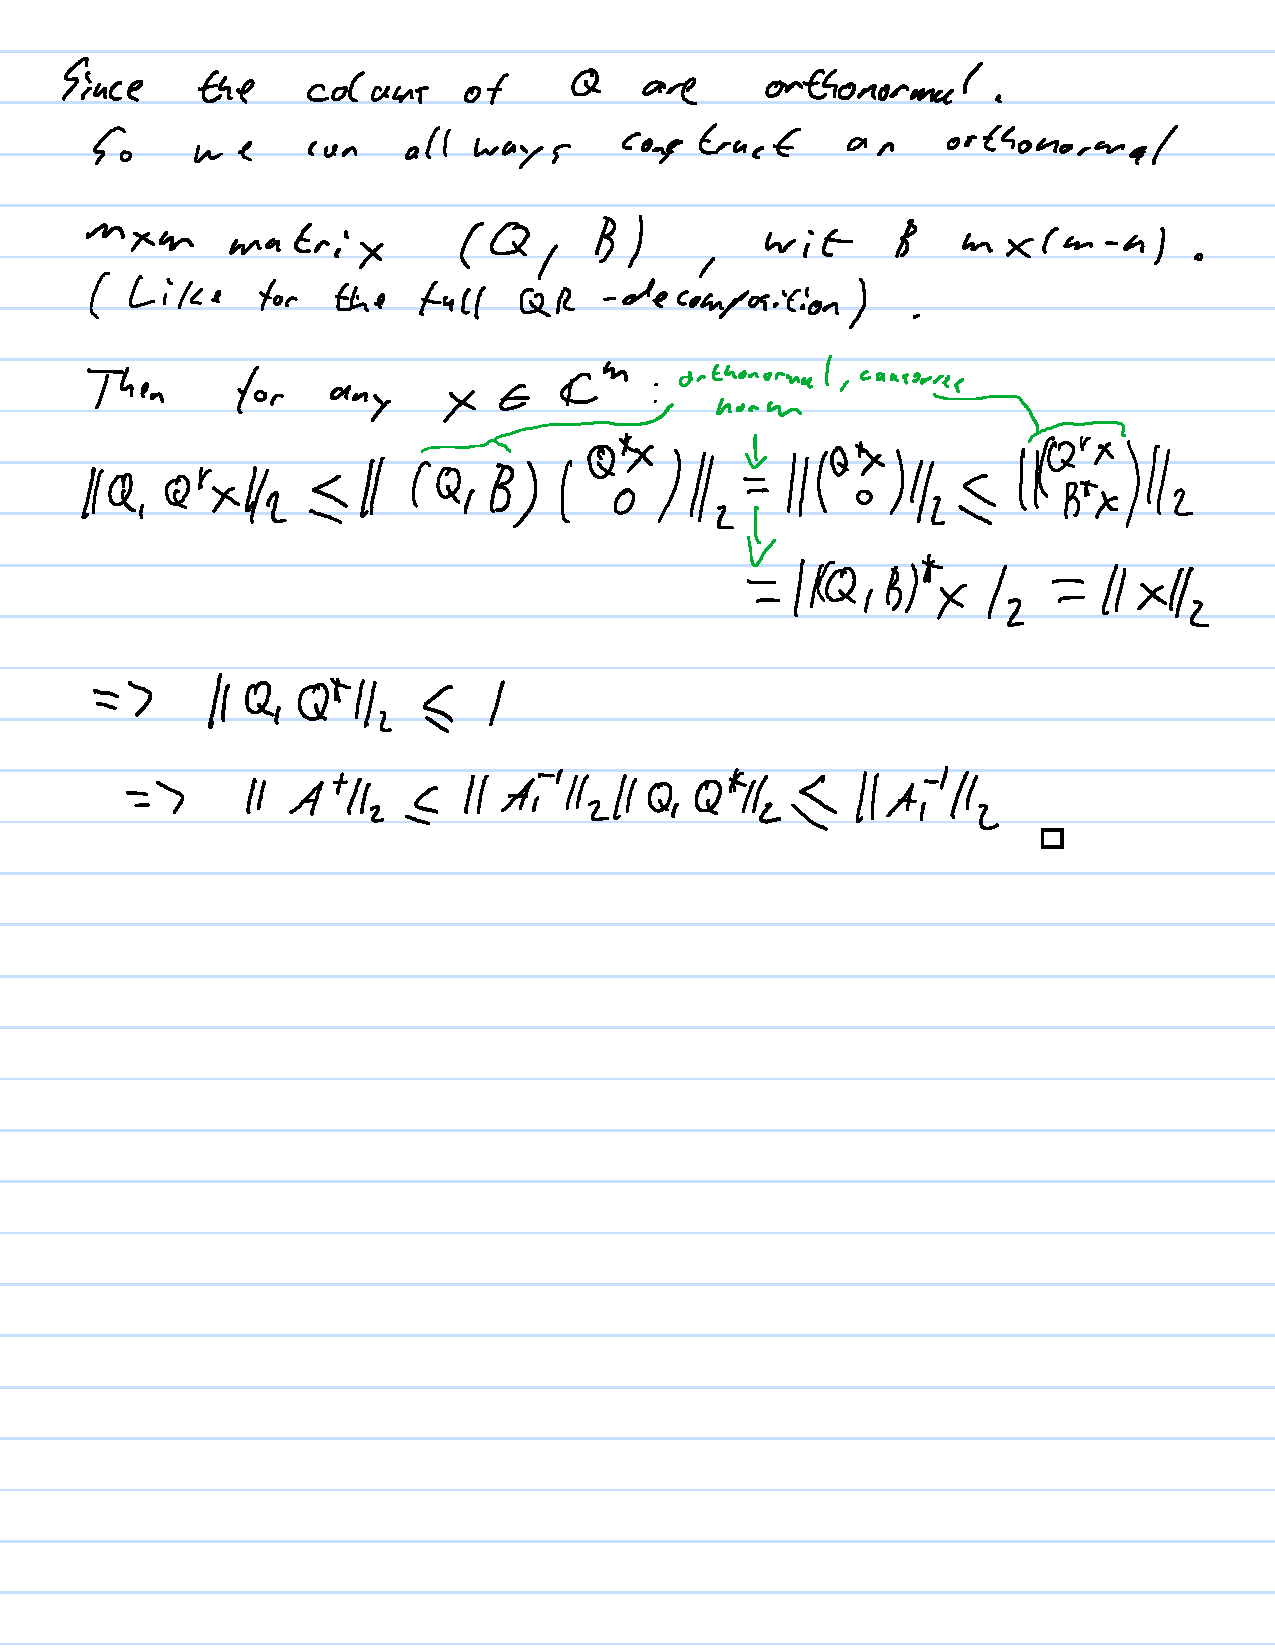
\includepdf{../1/1_2.pdf}

\section*{2.}
\begin{figure}
  \centering
  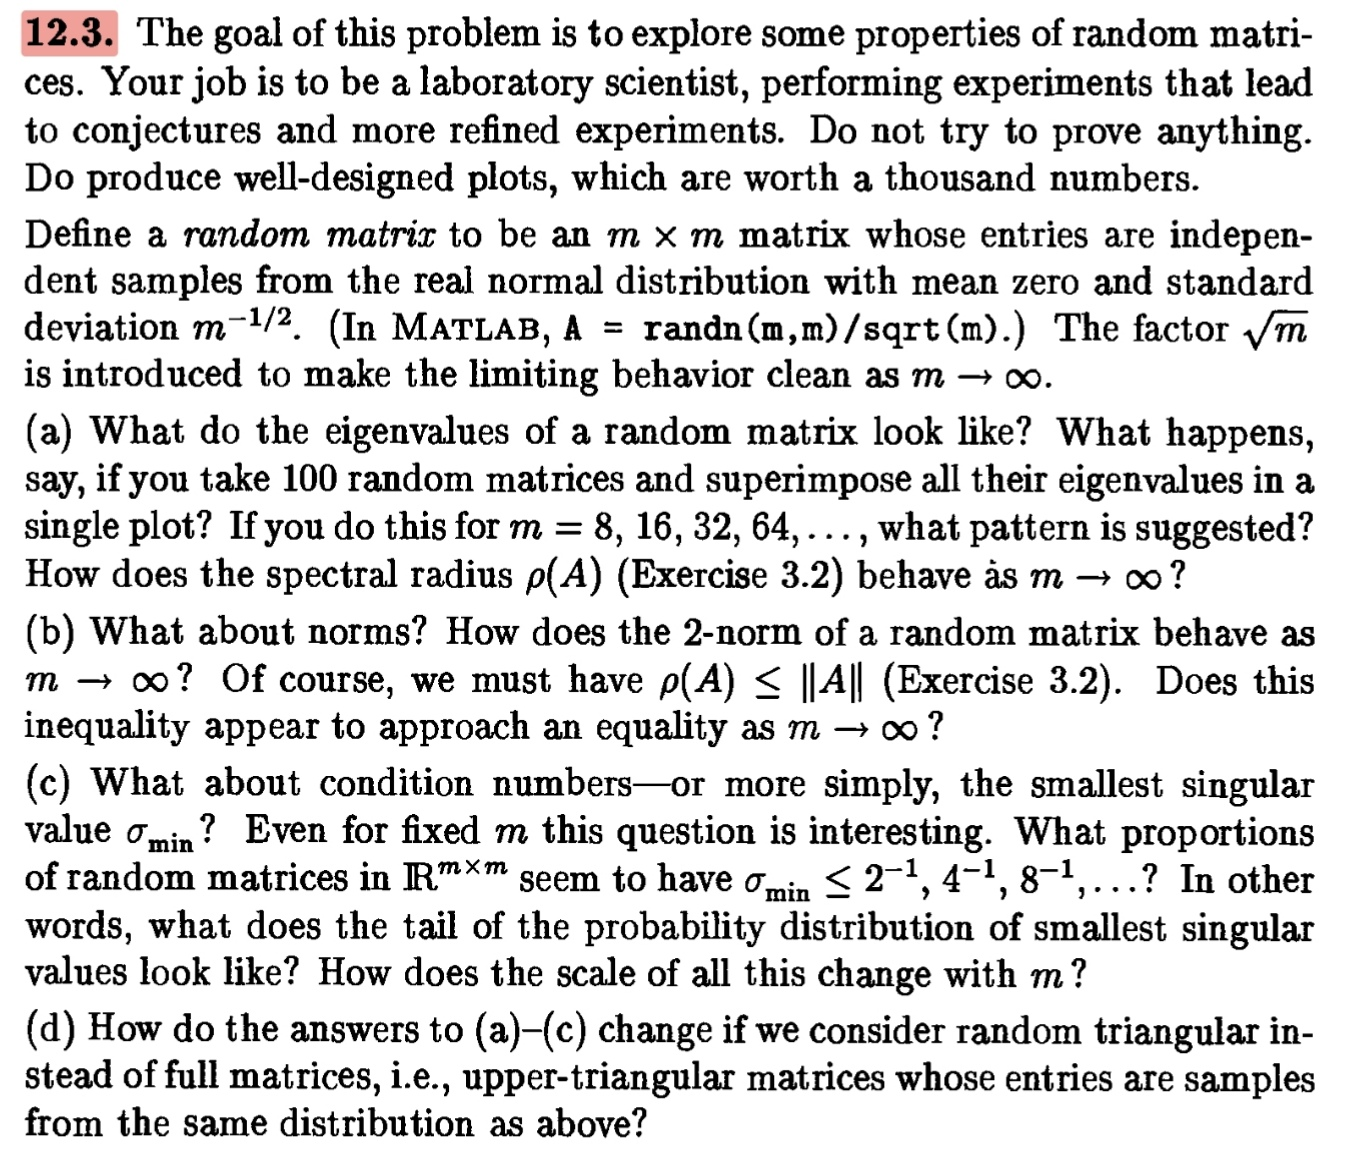
\includegraphics[width=\textwidth]{../2/12_3.jpg}
\end{figure}

For all of the sub-parts of this part I chose $m$ to be all powers of 2 from 2
to 512. For each $m$ I generate $10^{4}$ matrices, which is by no means large
enough to draw any statistically relevant conclusions. The results dependent on
$m$ for \textbf{(a)} to \textbf{(c)} are shown in Figure~\ref{fig:a-c} and
Figure~\ref{fig:a-c_zoomed}.
\begin{figure}
  \centering
  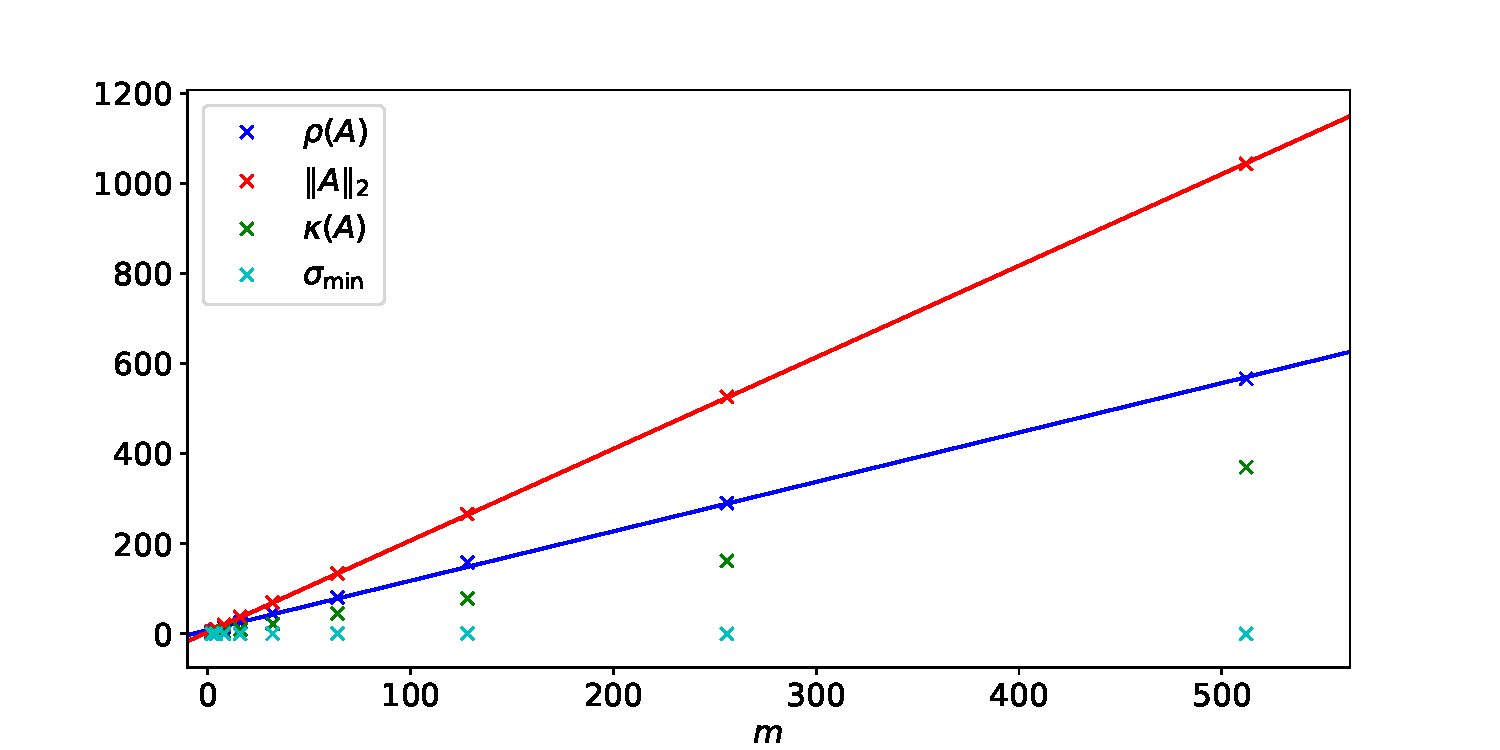
\includegraphics[width=\textwidth]{../2/norm_spectral_cond.pdf}
  \caption{The norm, spectral radius, condition number and smallest singular
  value out of a sample of square Gaussian random matrices in dependence of
  their dimension $m$.}
  \label{fig:a-c}
\end{figure}
\begin{figure}
  \centering
  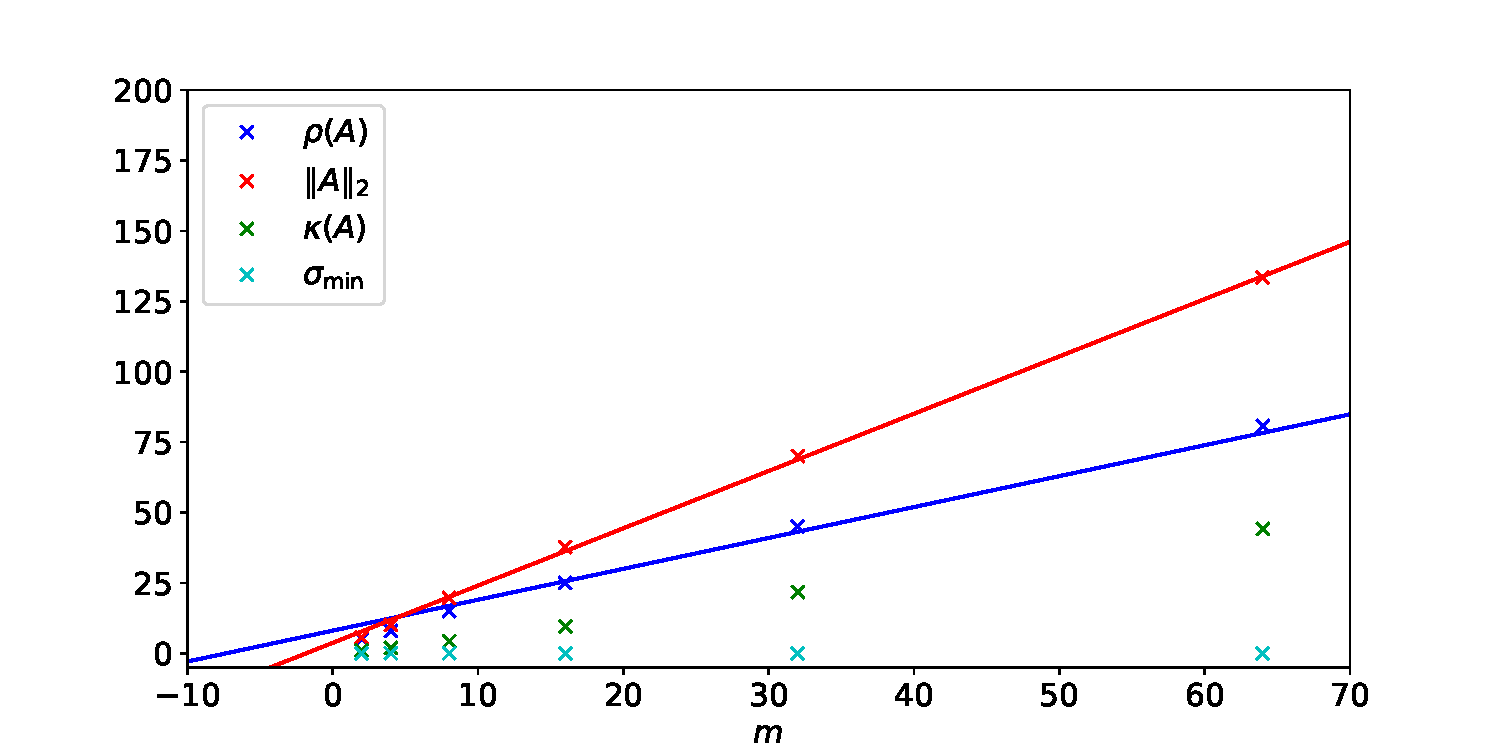
\includegraphics[width=\textwidth]{../2/norm_spectral_cond_zoomed.pdf}
  \caption{Zoomed in view for small $m$ of Figure~\ref{fig:a-c}.}
  \label{fig:a-c_zoomed}
\end{figure}

\FloatBarrier
\subsection*{(a)}
Plots of the complex plane with all eigenvalues for each $m$ are shown in
Figure~\ref{fig:evs_2} to Figure~\ref{fig:evs_512}. It is obvious, that most of
the eigenvalues seem to be almost uniformly distributed within a circle of
radius $m$. Meaning that there absolute value is most likely to be smaller or
equal than $m$ and that the probability of getting an eigenvalue with absolute
value $r \leq m$ increases with the square of $r$ until $r = m$ where it
suddenly falls off. However, real eigenvalues seem to be more likely than
eigenvalues close to the real axis and they also seem to be more likely to fall
outside of the circle (meaning their absolute value being larger than $m$).
This effect seems to be more pronounced for small $m$ and starts to
asymptotically disappear for large $m$ in relative terms. 

If I had the time I would look at the PDFs of the absolute value of the
eigenvalues and their complex phase. As mentioned before I would expect a
square distribution for the absolute value with a steep cut-off at $m$. For the
distribution of complex phase I would expect a mostly uniform distribution,
with a slight peak at 0 and small dips close around it.

\begin{figure}
  \centering
  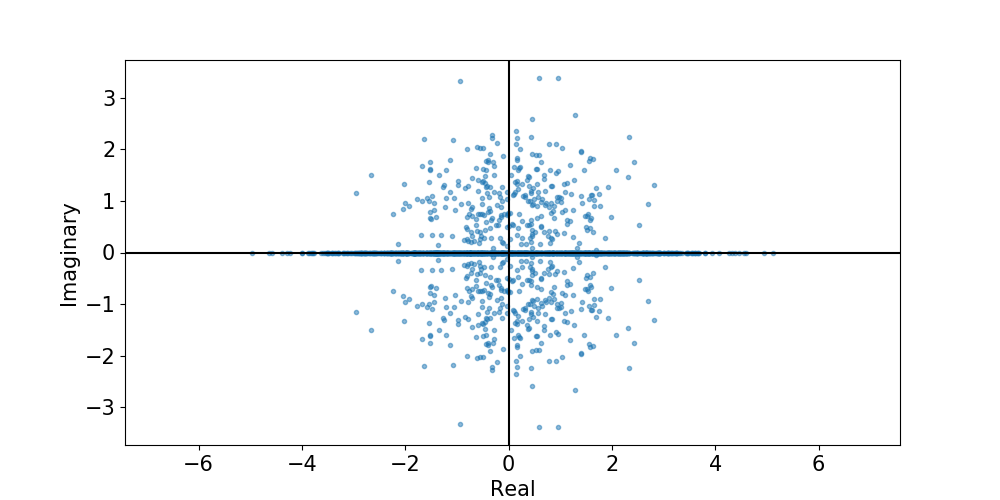
\includegraphics[width=\textwidth]{../2/square_evs/2.png}
  \caption{All eigenvalues of the sample with $m=2$.}
  \label{fig:evs_2}
\end{figure}
\begin{figure}
  \centering
  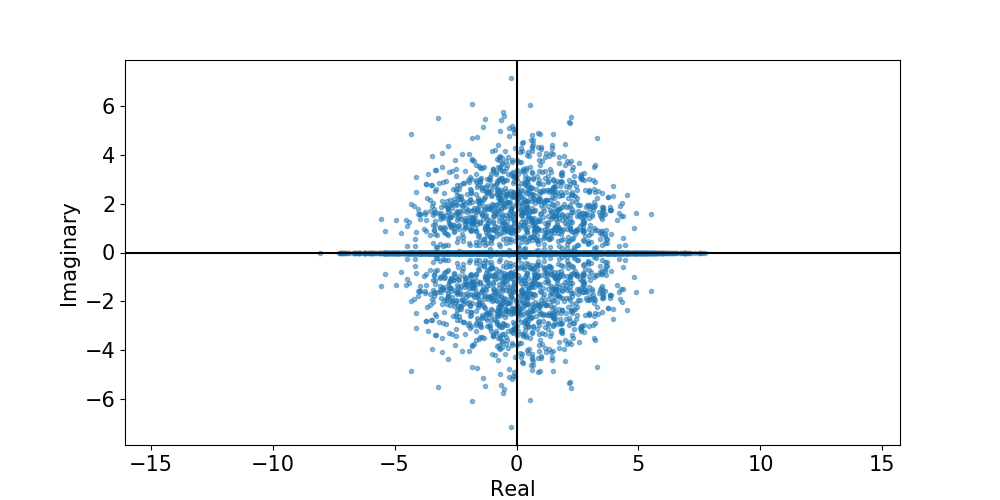
\includegraphics[width=\textwidth]{../2/square_evs/4.png}
  \caption{All eigenvalues of the sample with $m=4$.}
  \label{fig:evs_4}
\end{figure}
\begin{figure}
  \centering
  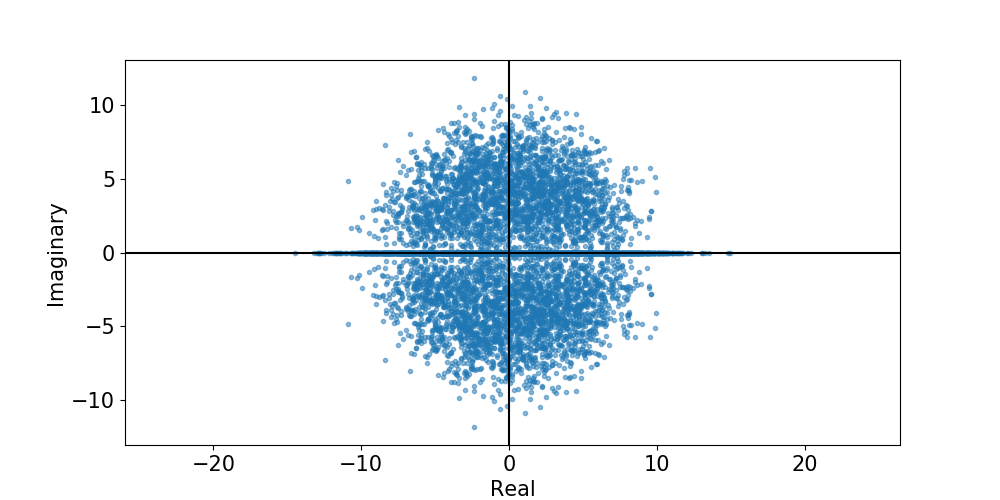
\includegraphics[width=\textwidth]{../2/square_evs/8.png}
  \caption{All eigenvalues of the sample with $m=8$.}
  \label{fig:evs_8}
\end{figure}
\begin{figure}
  \centering
  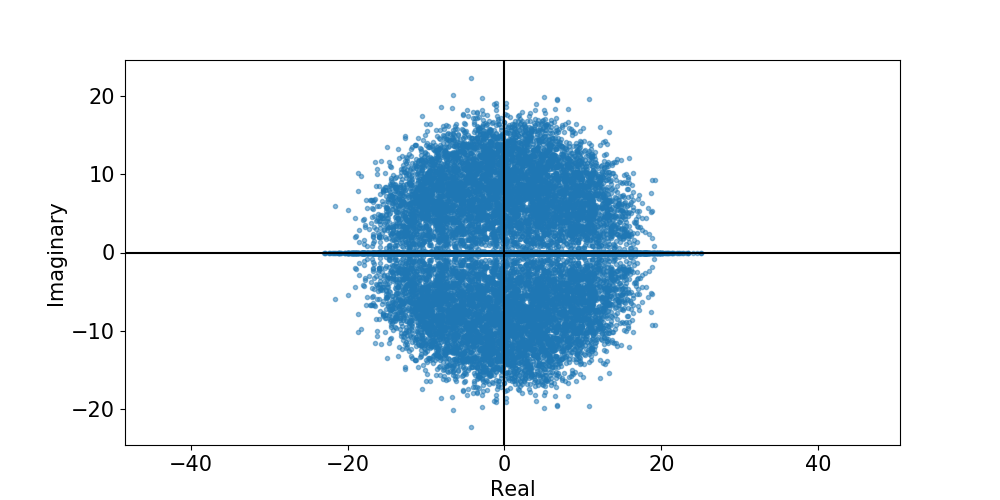
\includegraphics[width=\textwidth]{../2/square_evs/16.png}
  \caption{All eigenvalues of the sample with $m=16$.}
  \label{fig:evs_16}
\end{figure}
\begin{figure}
  \centering
  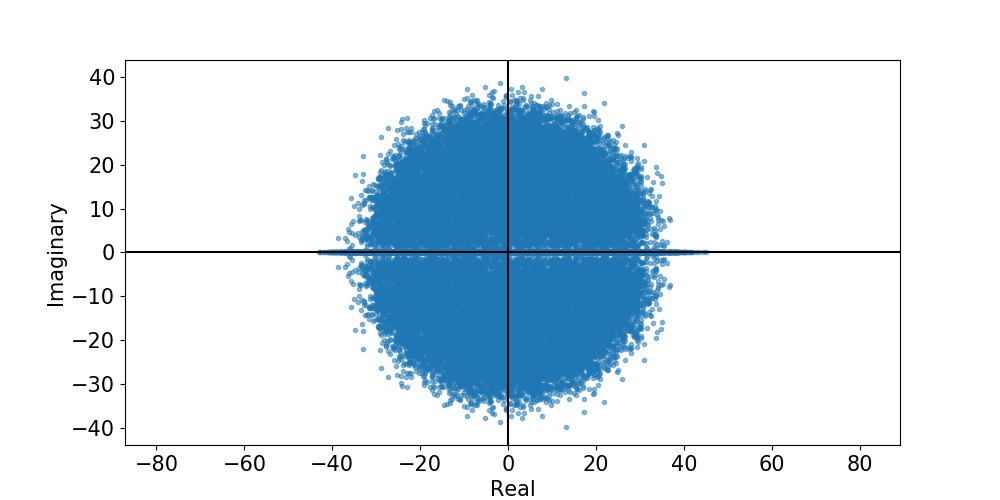
\includegraphics[width=\textwidth]{../2/square_evs/32.png}
  \caption{All eigenvalues of the sample with $m=32$.}
  \label{fig:evs_32}
\end{figure}
\begin{figure}
  \centering
  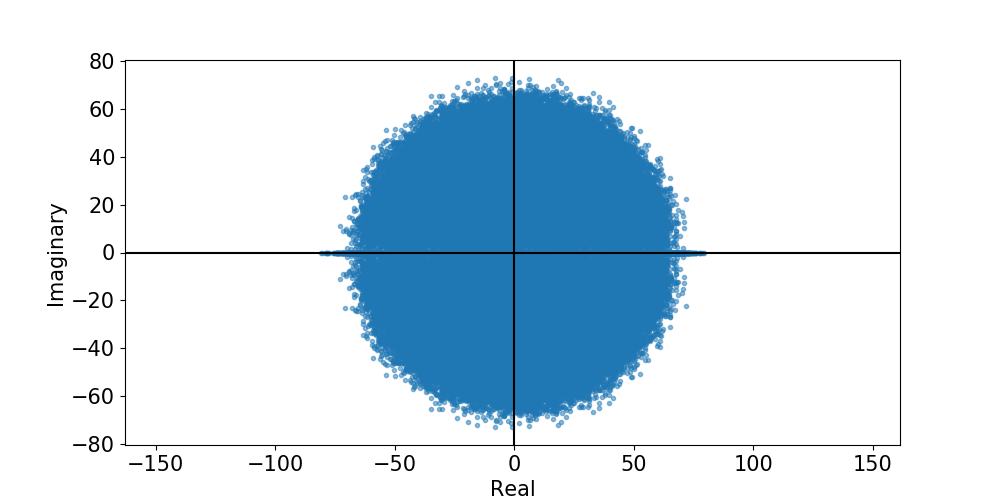
\includegraphics[width=\textwidth]{../2/square_evs/64.png}
  \caption{All eigenvalues of the sample with $m=64$.}
  \label{fig:evs_64}
\end{figure}
\begin{figure}
  \centering
  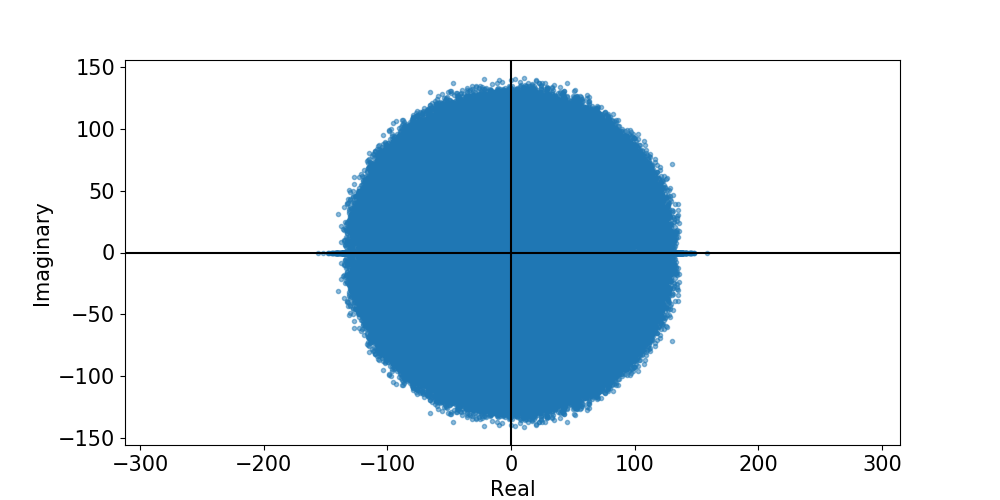
\includegraphics[width=\textwidth]{../2/square_evs/128.png}
  \caption{All eigenvalues of the sample with $m=128$.}
  \label{fig:evs_128}
\end{figure}
\begin{figure}
  \centering
  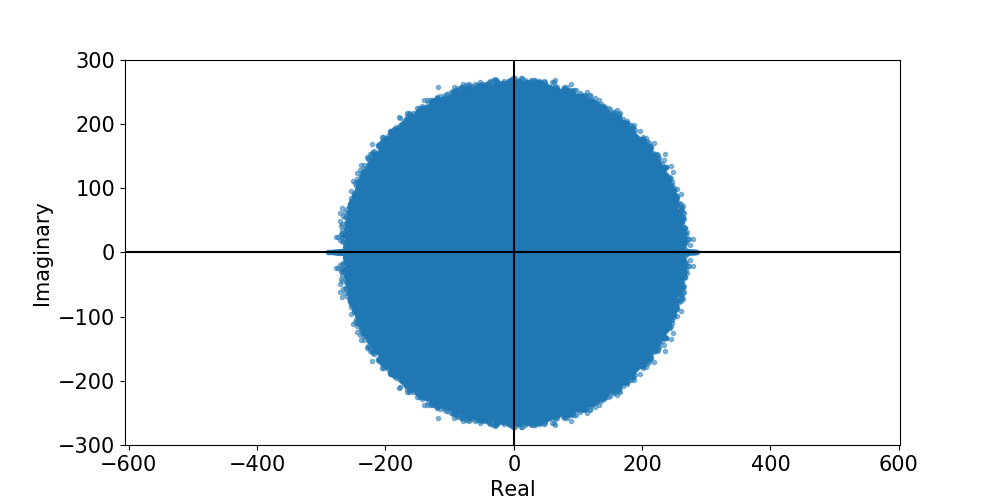
\includegraphics[width=\textwidth]{../2/square_evs/256.png}
  \caption{All eigenvalues of the sample with $m=256$.}
  \label{fig:evs_256}
\end{figure}
\begin{figure}
  \centering
  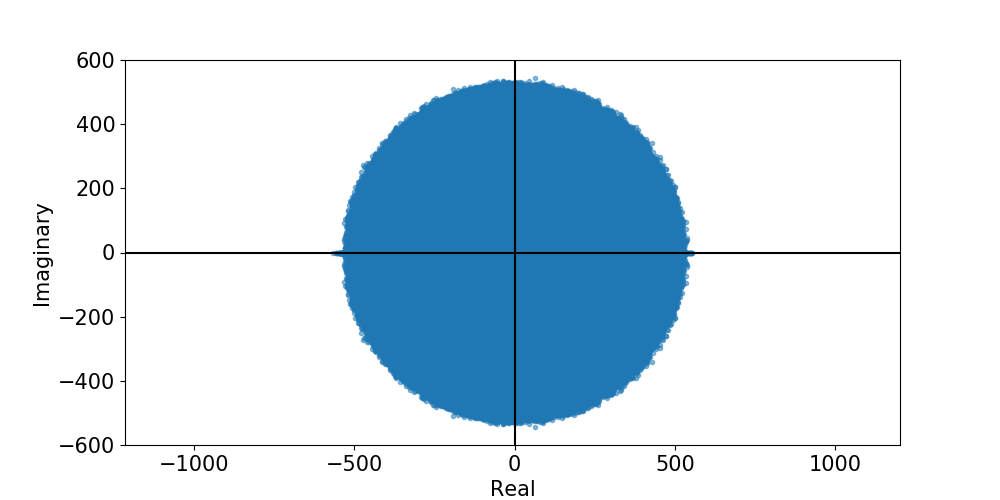
\includegraphics[width=\textwidth]{../2/square_evs/512.png}
  \caption{All eigenvalues of the sample with $m=512$.}
  \label{fig:evs_512}
\end{figure}

\FloatBarrier
\subsection*{b)}
I know we are not supposed to prove anything, but the inequality
\begin{equation}
  \rho(A) \leq \Vert A\Vert
\end{equation}
could not possibly approach an equality for $m \rightarrow \infty$ because it in
fact holds true for the case $m=1$ (which is immediately obvious). The
inequality grows larger with $m$ as it can be seen in Figure~\ref{fig:a-c}.

Both the L2 norm and the spectral radius appear to grow proportionally with
$m$, as the linear regressions shown in Figure~\ref{fig:a-c} suggest. I find
\begin{equation}
  \rho(A) \approx 1.10\cdot m + 8.10
\end{equation}
with a standard error of $10^{-2}$ and
\begin{equation}
  \Vert A \Vert \approx 2.033\cdot m + 3.762
\end{equation}
with a standard error of $3\cdot 10^{-3}$.

\FloatBarrier
\subsection*{(c)}
The minimal condition numbers $\kappa(A)$ and smallest singular values
$\sigma_\textup{min}$ for the different samples with varied $m$ are also shown
in Figure~\ref{fig:a-c}. They both do not seem to follow any obvious trend.
However, especially for the smallest singular values the result is extremely
volatile between runs of the script. A zoomed in view is given by
Figure~\ref{fig:sig_min}. This figure can not be used to draw any conclusions
as the statistics are not sufficient. 
\begin{figure}
  \centering
  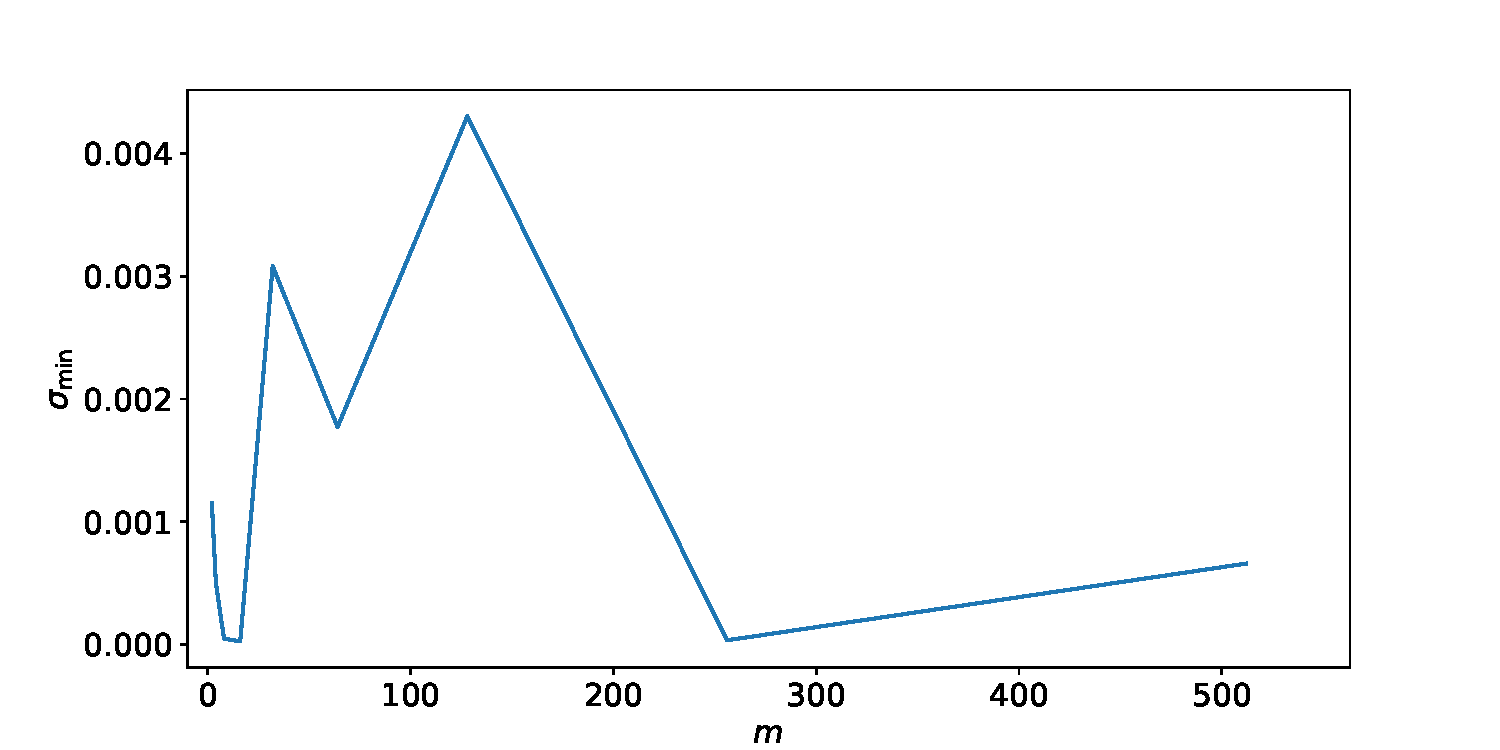
\includegraphics[width=\textwidth]{../2/sigma_min.pdf}
  \caption{The minimal singular values of all samples. This figure is just an
  example and looks very different for every run.}
  \label{fig:sig_min}
\end{figure}

To learn about how the minimal singular values are effected by $m$, it makes a
lot more sense to look at the distributions as suggested by the assignment.
Figure~\ref{fig:sigma_min_ECDF_2} to Figure~\ref{fig:sigma_min_ECDF_512} show
the empirical cumulative density functions of the smallest singular values for
all matrices in the respective sample. The distribution does not seem to be
effected by $m$.

\begin{figure}
  \centering
  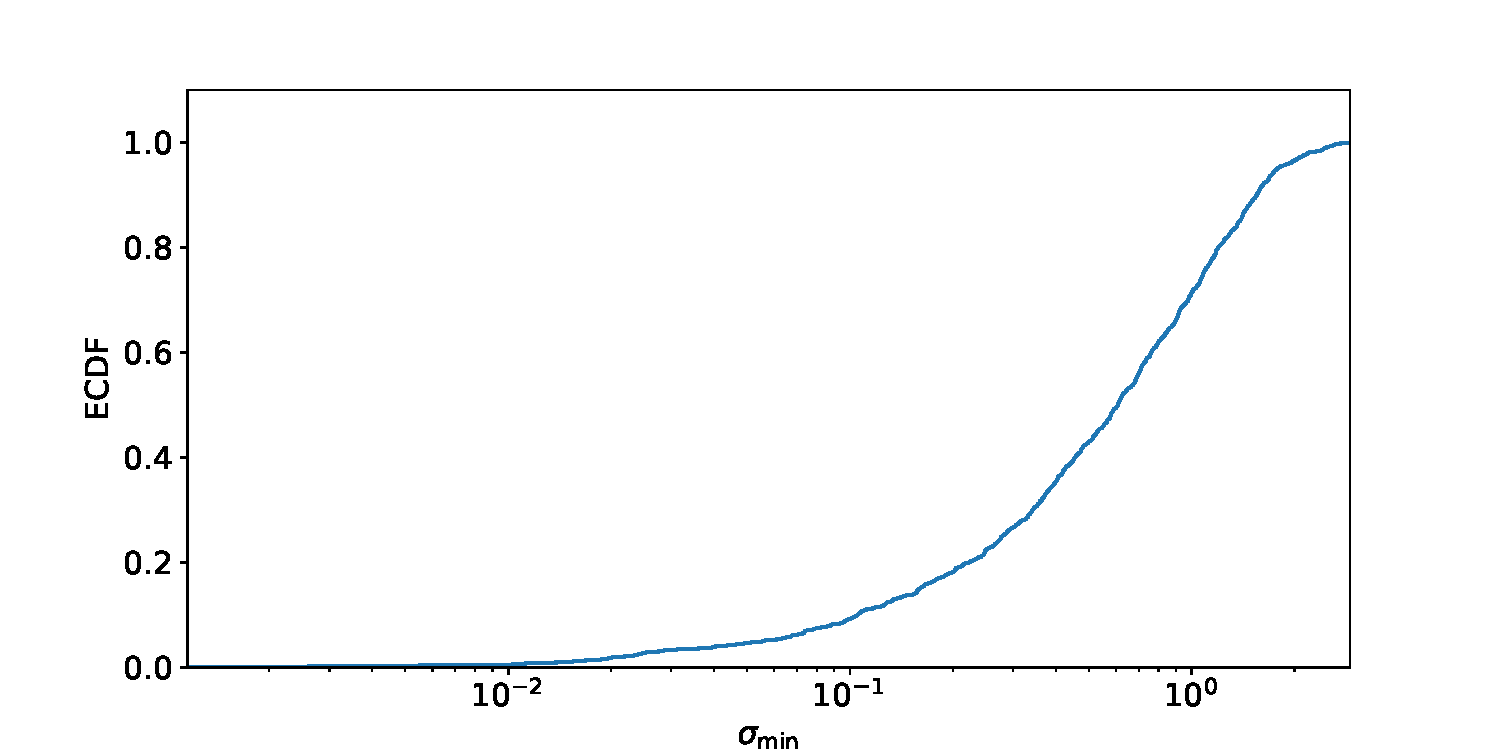
\includegraphics[width=\textwidth]{../2/square_ecdf/2.pdf}
  \caption{ECDF of the smallest singular values for all matrices in the sample with $m=2$.}
  \label{fig:sigma_min_ECDF_2}
\end{figure}
\begin{figure}
  \centering
  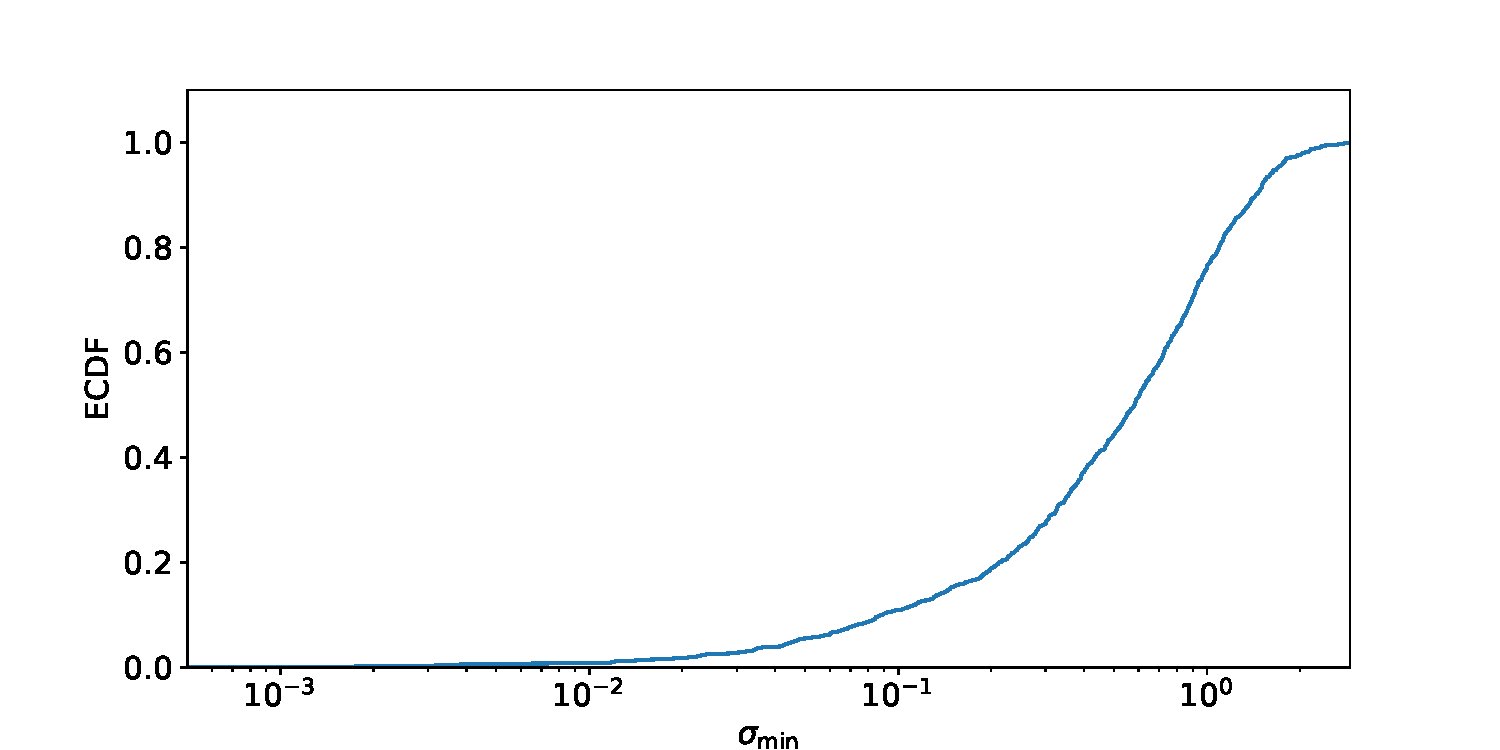
\includegraphics[width=\textwidth]{../2/square_ecdf/4.pdf}
  \caption{ECDF of the smallest singular values for all matrices in the sample with $m=4$.}
  \label{fig:sigma_min_ECDF_4}
\end{figure}
\begin{figure}
  \centering
  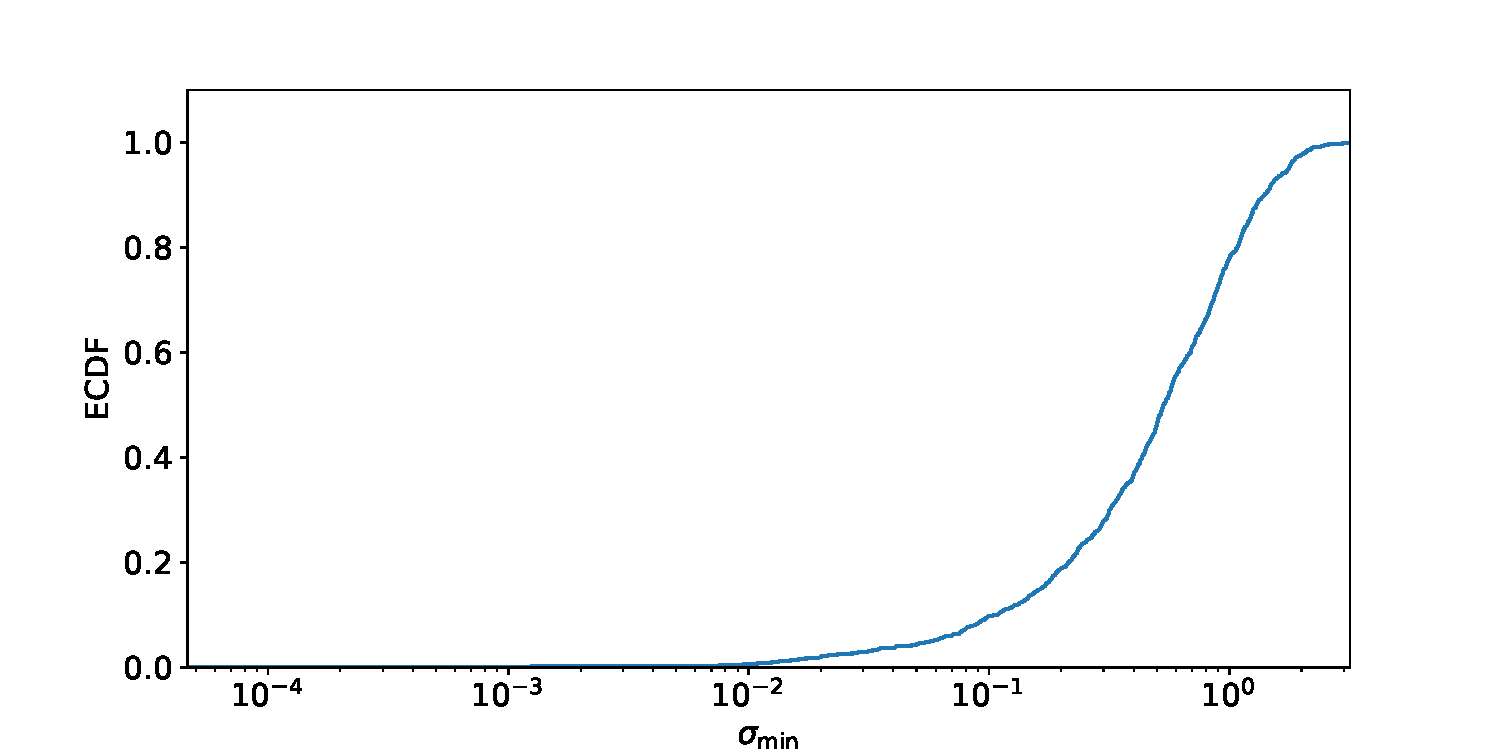
\includegraphics[width=\textwidth]{../2/square_ecdf/8.pdf}
  \caption{ECDF of the smallest singular values for all matrices in the sample with $m=8$.}
  \label{fig:sigma_min_ECDF_8}
\end{figure}
\begin{figure}
  \centering
  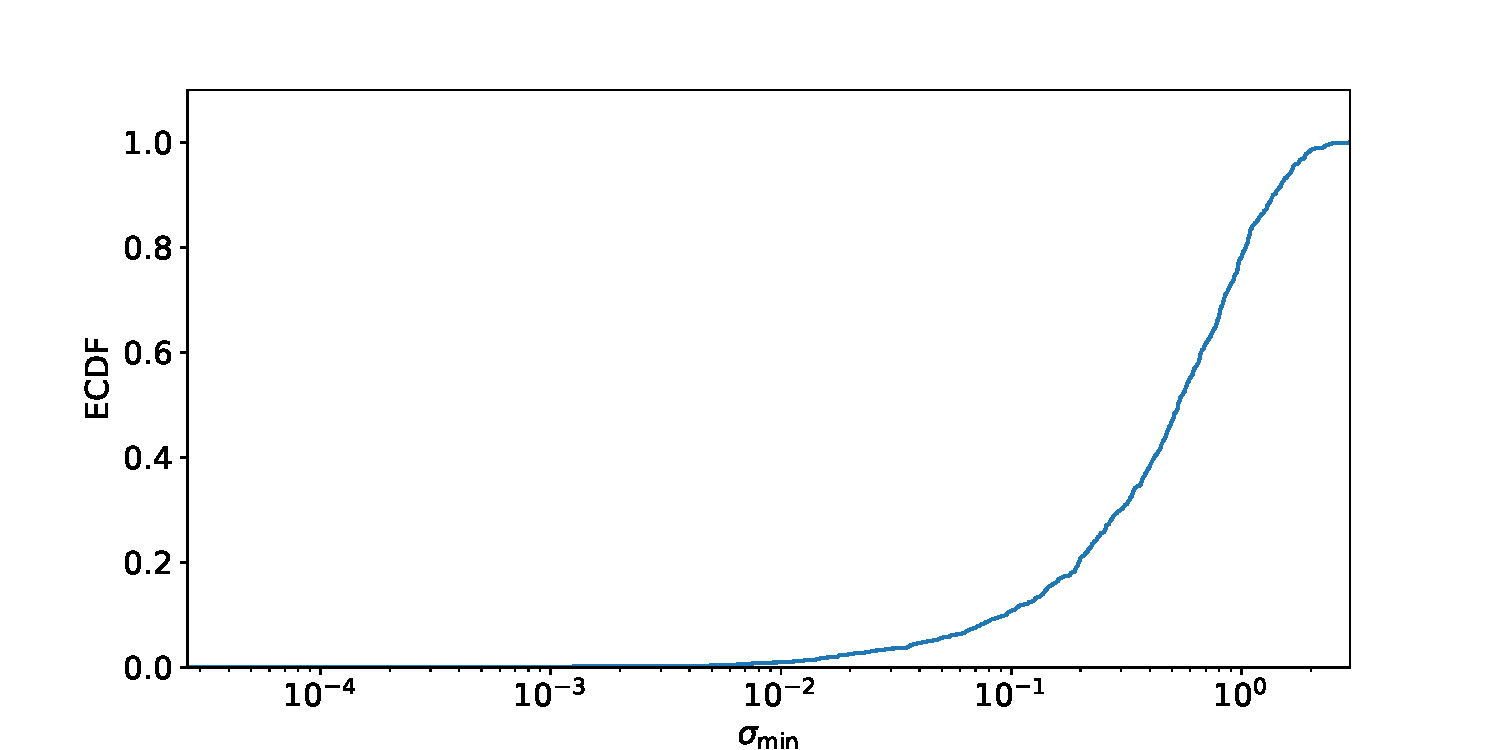
\includegraphics[width=\textwidth]{../2/square_ecdf/16.pdf}
  \caption{ECDF of the smallest singular values for all matrices in the sample with $m=16$.}
  \label{fig:sigma_min_ECDF_16}
\end{figure}
\begin{figure}
  \centering
  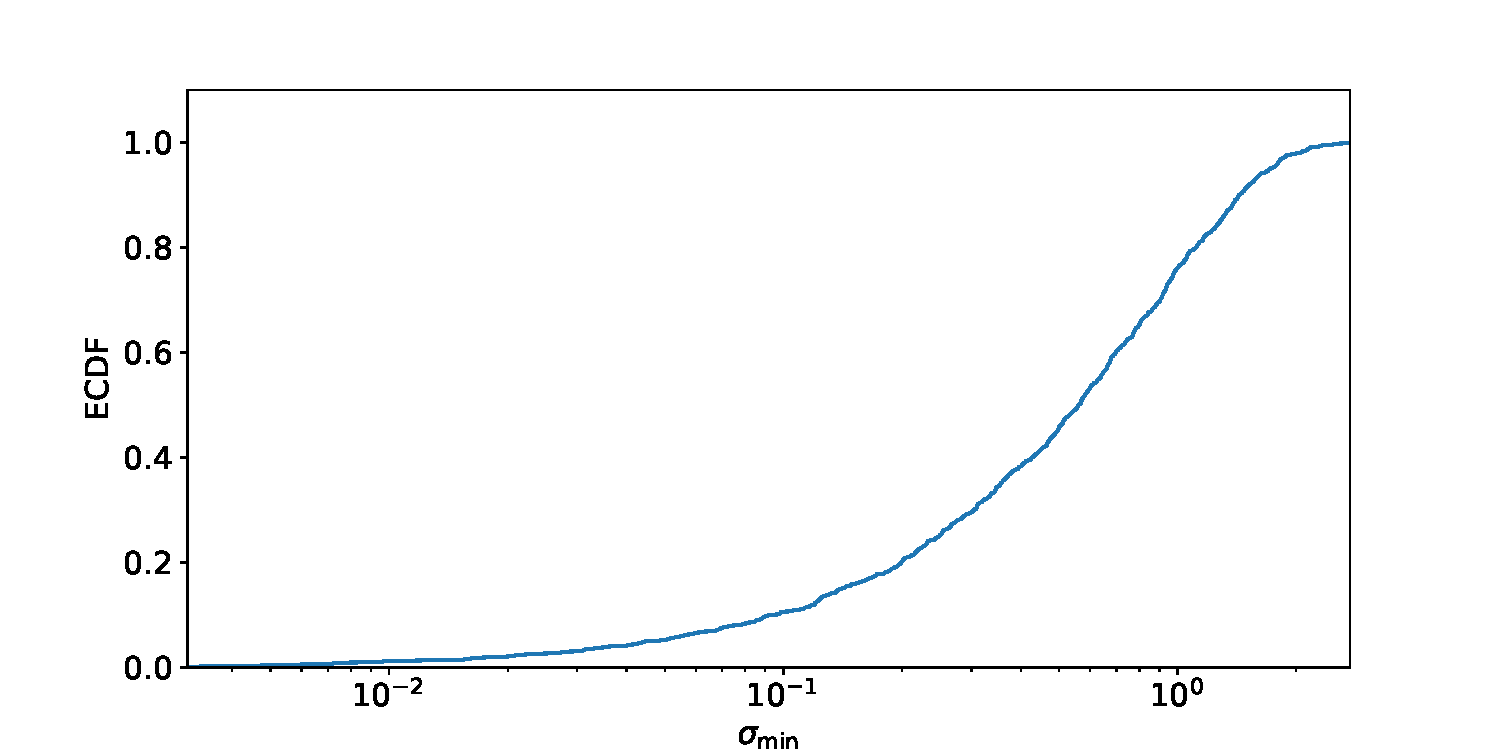
\includegraphics[width=\textwidth]{../2/square_ecdf/32.pdf}
  \caption{ECDF of the smallest singular values for all matrices in the sample with $m=32$.}
  \label{fig:sigma_min_ECDF_32}
\end{figure}
\begin{figure}
  \centering
  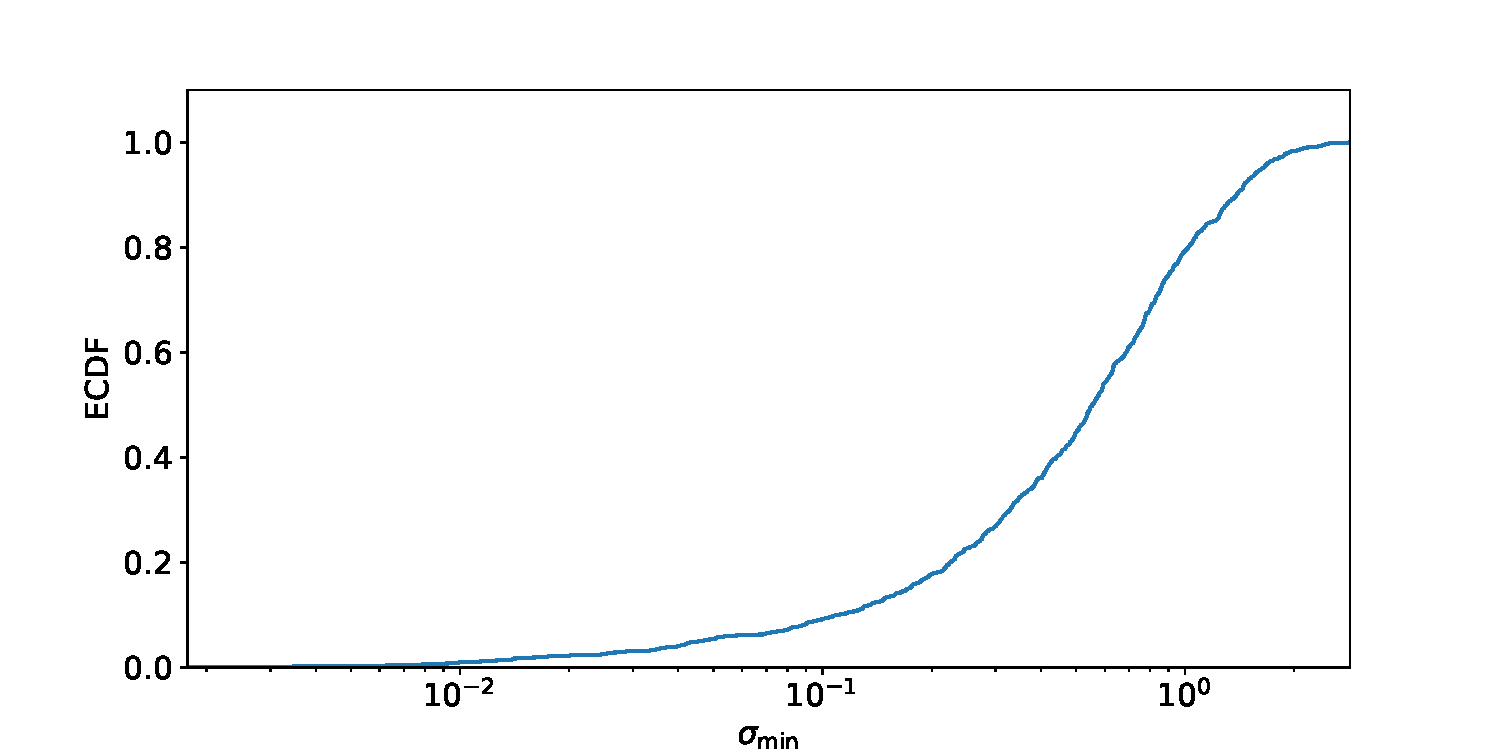
\includegraphics[width=\textwidth]{../2/square_ecdf/64.pdf}
  \caption{ECDF of the smallest singular values for all matrices in the sample with $m=64$.}
  \label{fig:sigma_min_ECDF_64}
\end{figure}
\begin{figure}
  \centering
  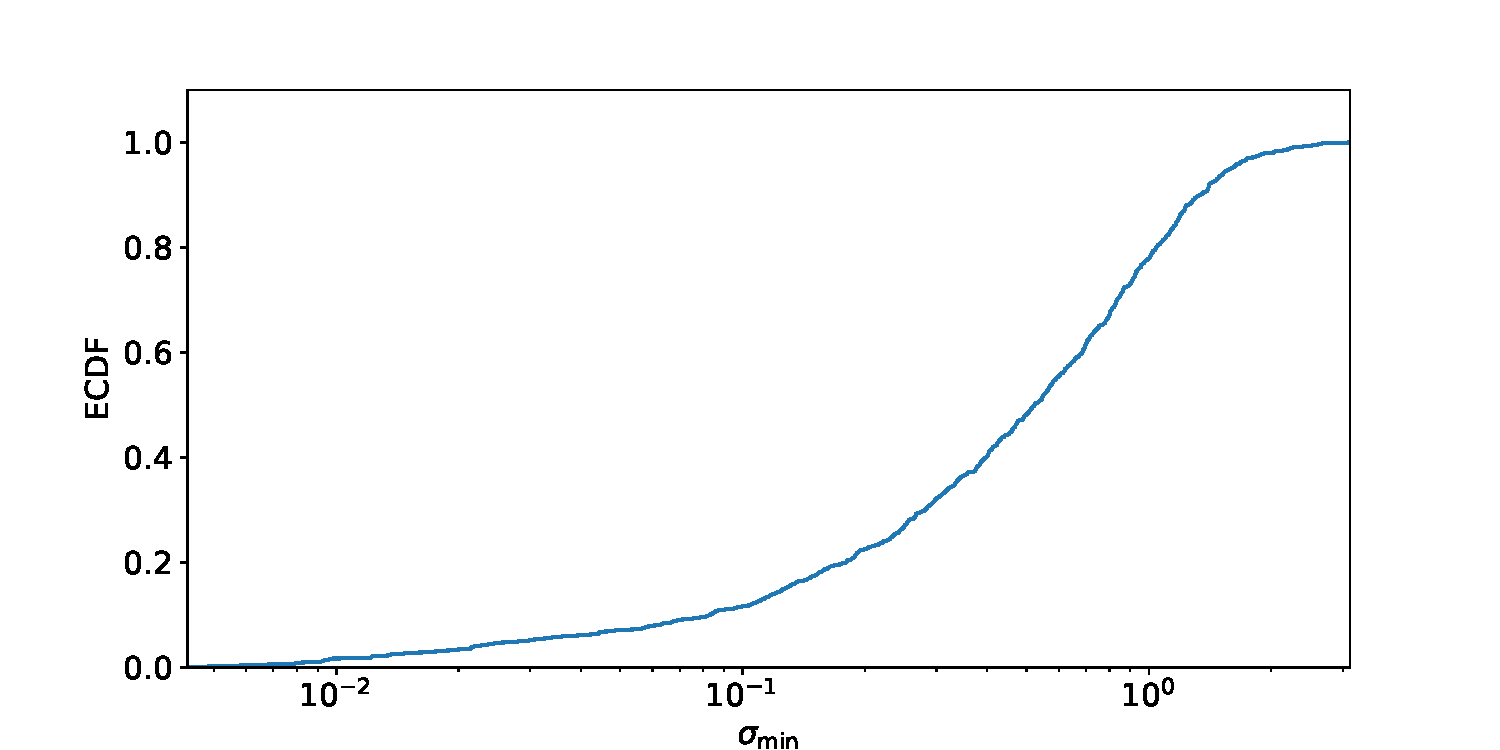
\includegraphics[width=\textwidth]{../2/square_ecdf/128.pdf}
  \caption{ECDF of the smallest singular values for all matrices in the sample with $m=128$.}
  \label{fig:sigma_min_ECDF_128}
\end{figure}
\begin{figure}
  \centering
  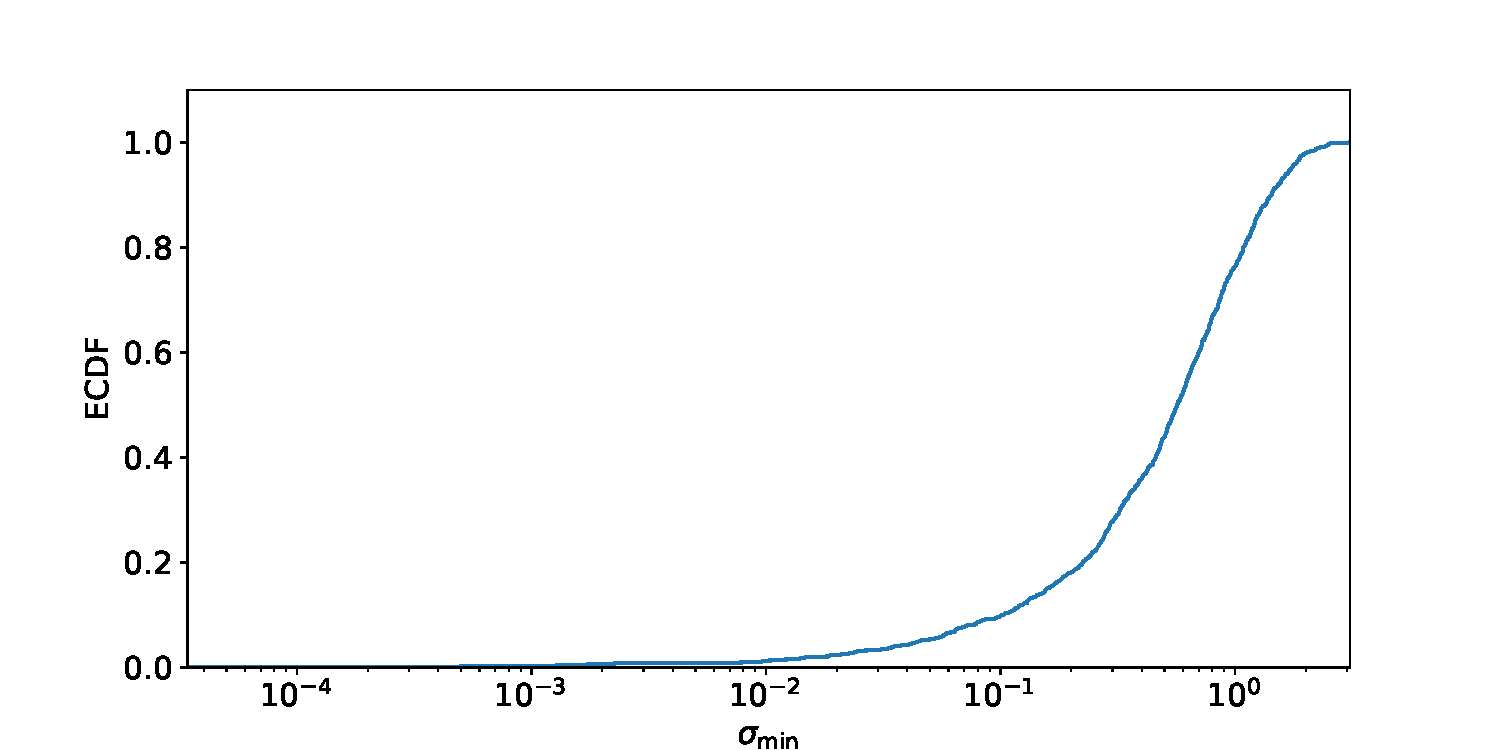
\includegraphics[width=\textwidth]{../2/square_ecdf/256.pdf}
  \caption{ECDF of the smallest singular values for all matrices in the sample with $m=256$.}
  \label{fig:sigma_min_ECDF_256}
\end{figure}
\begin{figure}
  \centering
  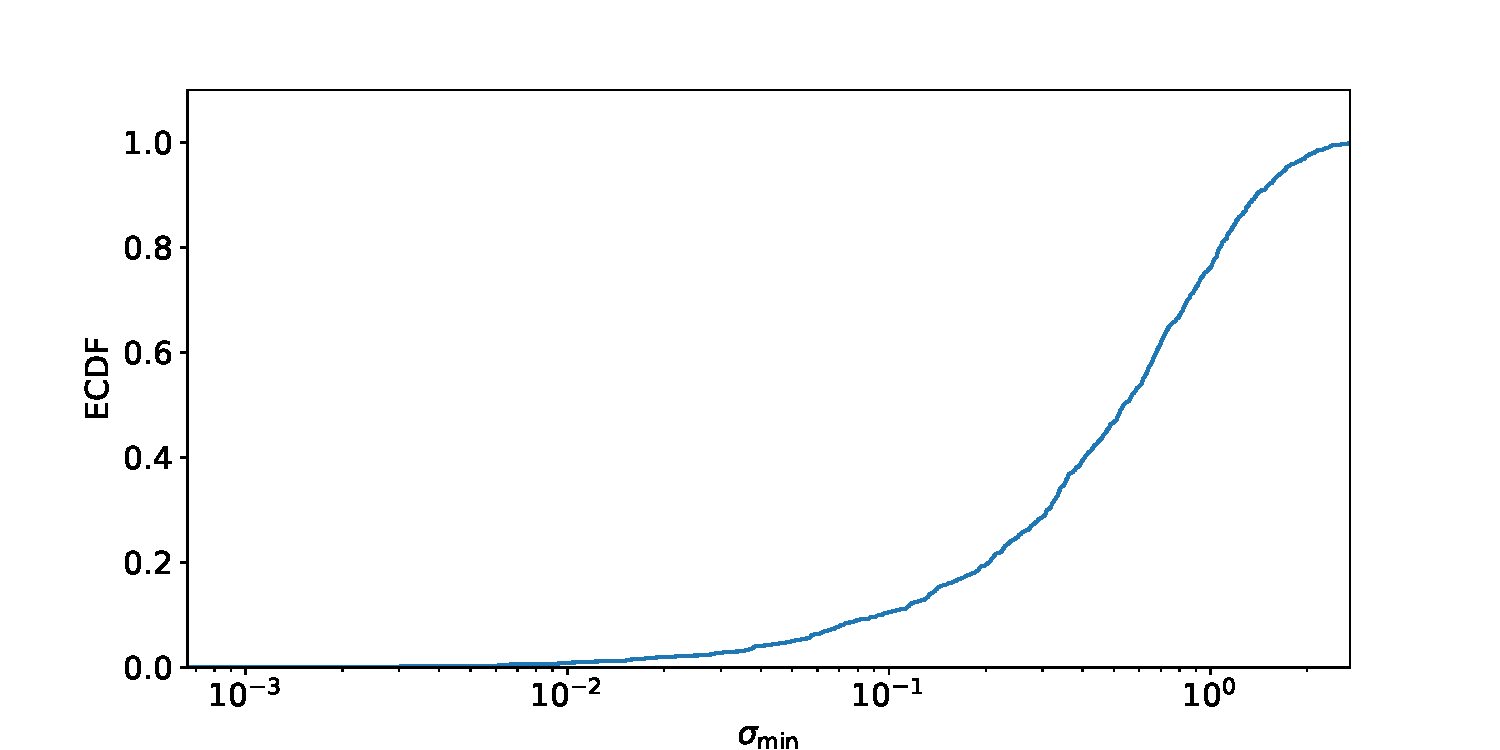
\includegraphics[width=\textwidth]{../2/square_ecdf/512.pdf}
  \caption{ECDF of the smallest singular values for all matrices in the sample with $m=512$.}
  \label{fig:sigma_min_ECDF_512}
\end{figure}

\FloatBarrier
\subsection*{(d)}
Okay now let's see what changes for upper triangular Guassian random matrices.
Obviously now we only get real eigenvalues. So the plots from \textbf{(a)} are
a waist of space and I won't include them here for that reason. However, the
behavior for eigenvalues on the real axis (so all of them here) seems the same
as for the square matrices.

The same plots as before are provided in Figure~\ref{fig:d_a-c} and
Figure~\ref{fig:d_a-c_zoomed} except that the condition numbers are plotted
seperately in Figure~\ref{fig:d_cond}, as they become to large to be shown in
the same plots. 
\begin{figure}
  \centering
  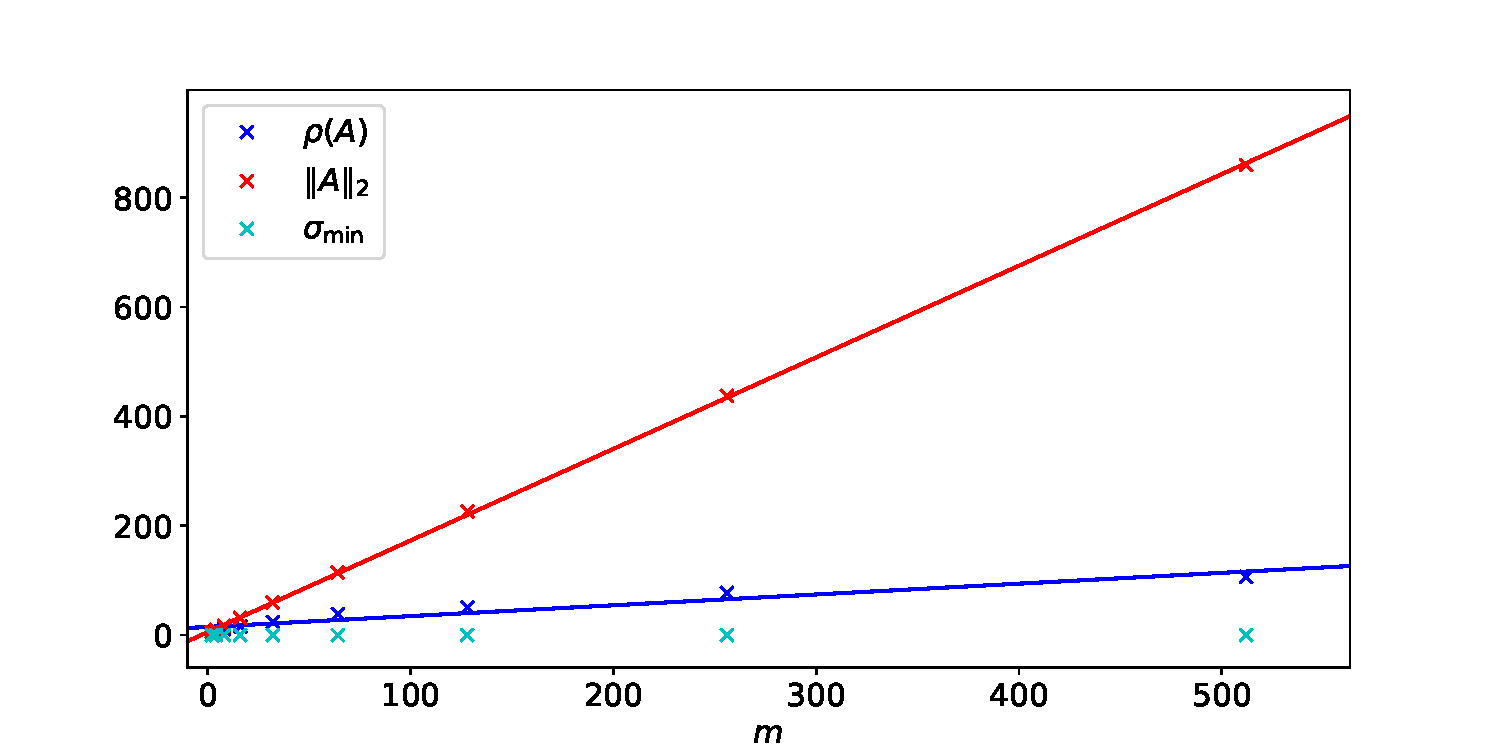
\includegraphics[width=\textwidth]{../2/triangular/norm_spectral.pdf}
  \caption{The norm and spectral index for triangular Gaussian random matrices
  with different $m$.}
  \label{fig:d_a-c}
\end{figure}
\begin{figure}
  \centering
  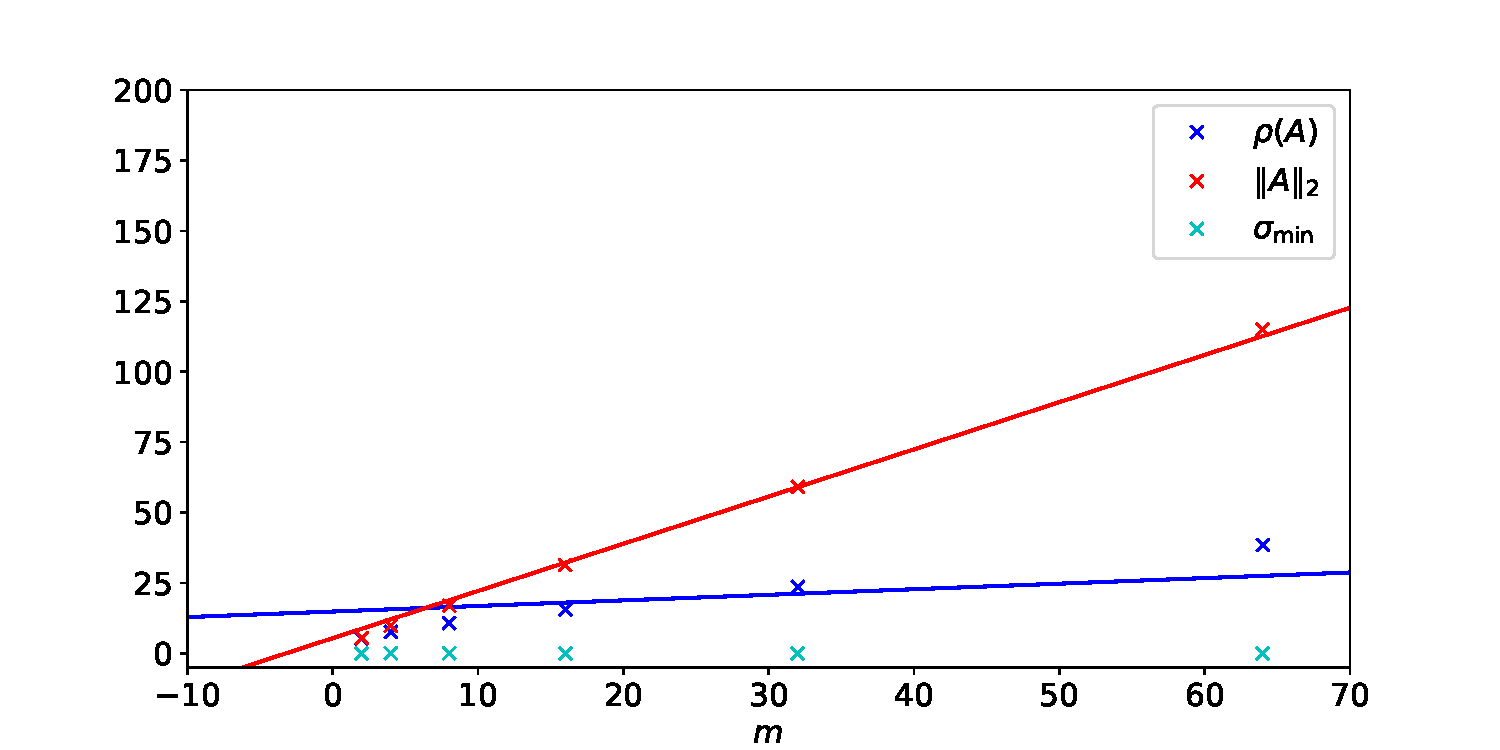
\includegraphics[width=\textwidth]{../2/triangular/norm_spectral_zoomed.pdf}
  \caption{Zoomed in view of Figure~\ref{fig:d_a-c}.}
  \label{fig:d_a-c_zoomed}
\end{figure}
\begin{figure}
  \centering
  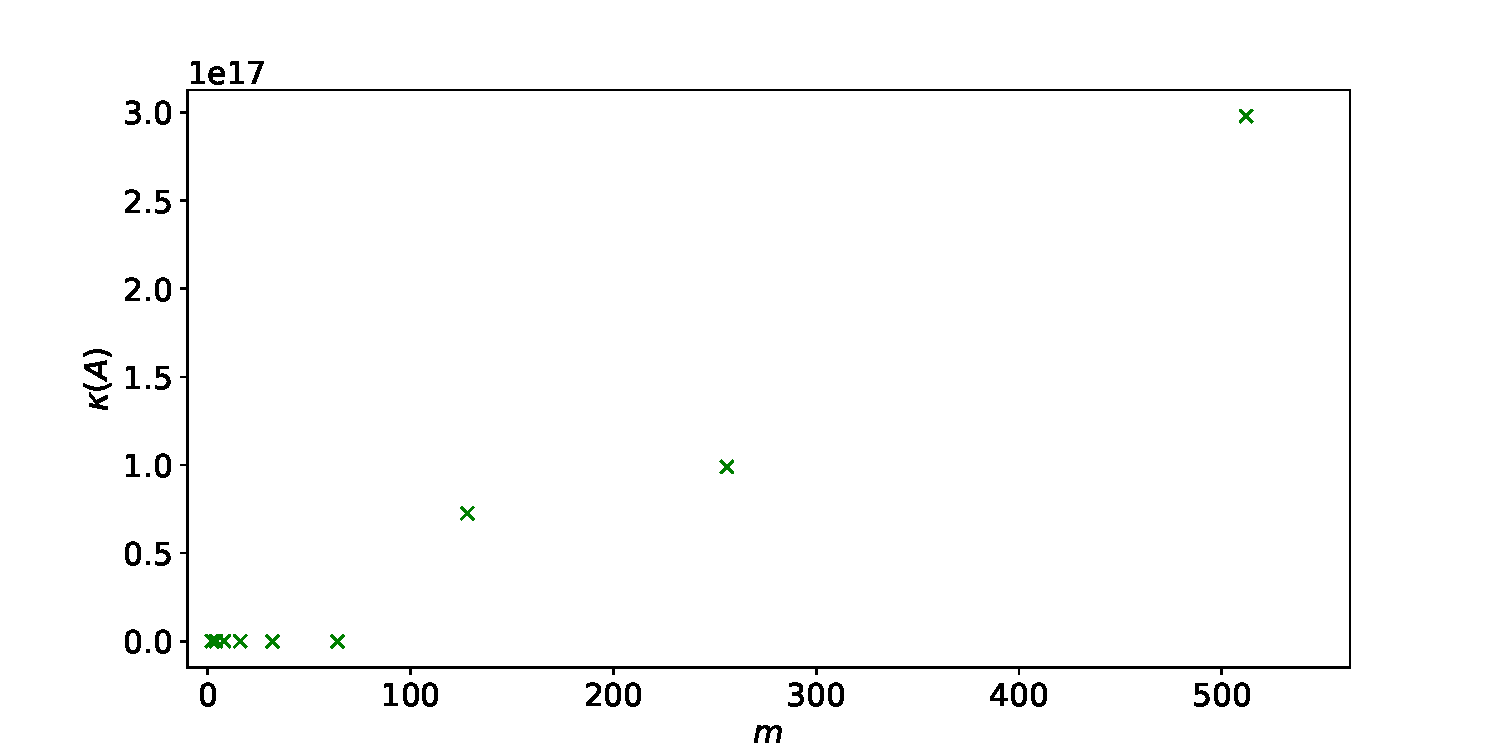
\includegraphics[width=\textwidth]{../2/triangular/cond.pdf}
  \caption{The condition numbers for the same triangular Gaussian random
  matrices.}
  \label{fig:d_cond}
\end{figure}

Again, both the L2 norm and the spectral radius appear to grow proportionally
with $m$, as the linear regressions shown in Figure~\ref{fig:a-c} suggest. Here
I find
\begin{equation}
  \rho(A) \approx 0.22\cdot m + 13.11
\end{equation}
with a standard error of $2\cdot 10^{-2}$ and
\begin{equation}
  \Vert A \Vert \approx 1.680\cdot m + 4.479
\end{equation}
with a standard error of $4\cdot 10^{-3}$. The general behavior is similar to
the square matrix case. It just appears as the spectral radius is now growing
significantly slower with $m$.

Where we do see a significant change is in the distribution of minimal singular
values. Again the empirical CDFs are shown in
Figure~\ref{fig:sigma_min_triangular_ECDF_2} to
Figure~\ref{fig:sigma_min_triangular_ECDF_512}. The tail of the distribution
for smallest singular values seems to extend and approach 0 as $m$ grows. We can
also see that by looking at Figure~\ref{fig:d_cond}: The triangular matrices
for large $m$ are significantly closer to being singular compared to their
square counterparts.
\begin{figure}
  \centering
  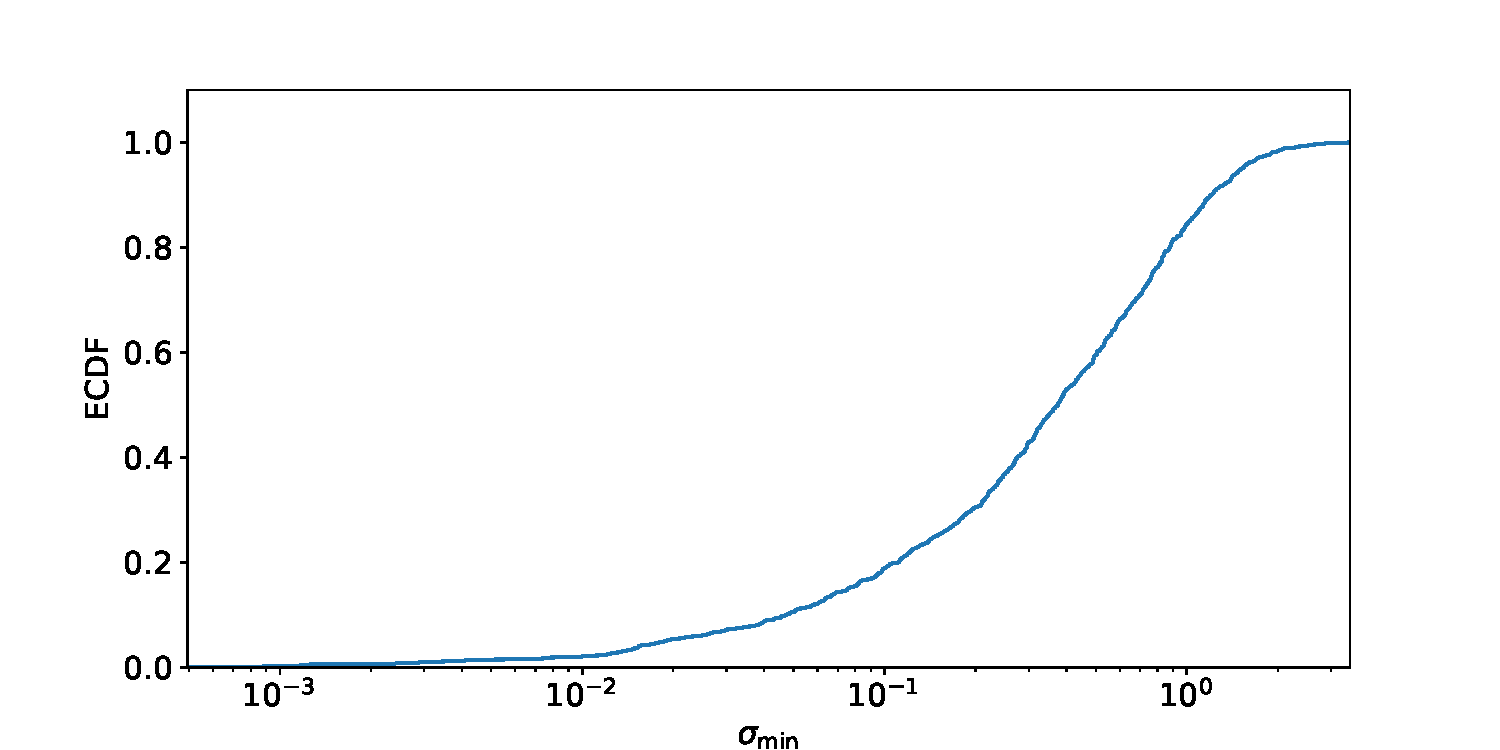
\includegraphics[width=\textwidth]{../2/triangular/ecdf/2.pdf}
  \caption{ECDF of the smallest singular values for all triangular matrices in
  the sample with $m=2$.}
  \label{fig:sigma_min_triangular_ECDF_2}
\end{figure}
\begin{figure}
  \centering
  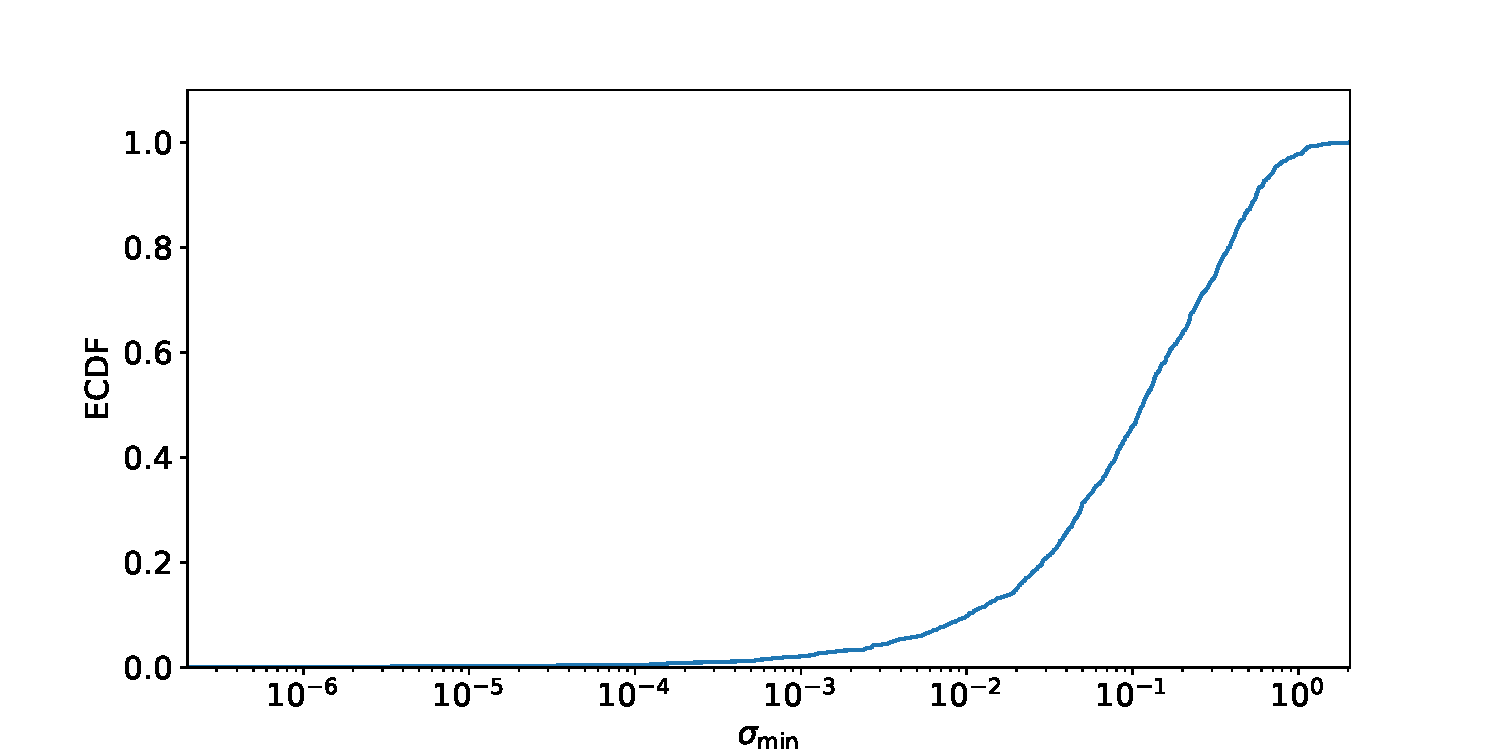
\includegraphics[width=\textwidth]{../2/triangular/ecdf/4.pdf}
  \caption{ECDF of the smallest singular values for all triangular matrices in
  the sample with $m=4$.}
  \label{fig:sigma_min_triangular_ECDF_4}
\end{figure}
\begin{figure}
  \centering
  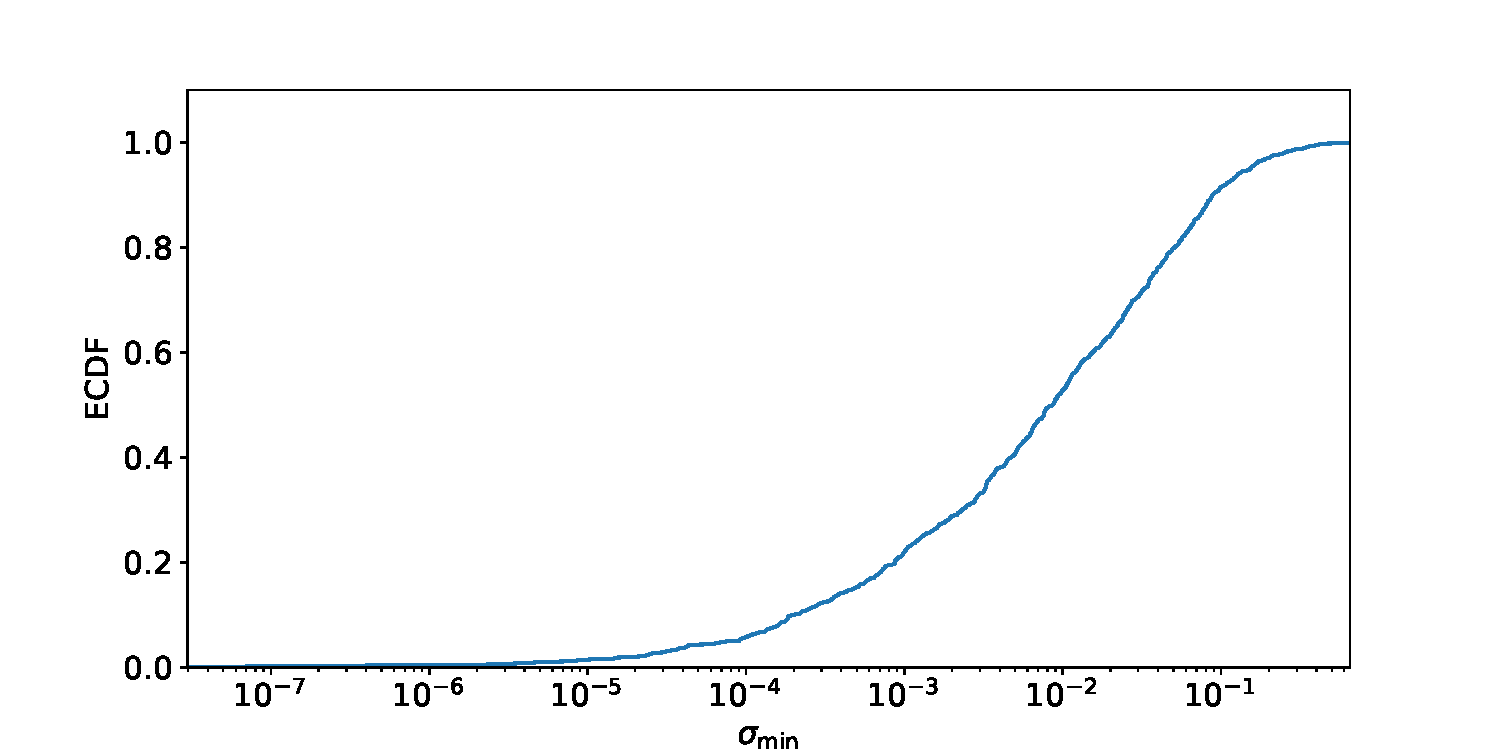
\includegraphics[width=\textwidth]{../2/triangular/ecdf/8.pdf}
  \caption{ECDF of the smallest singular values for all triangular matrices in
  the sample with $m=8$.}
  \label{fig:sigma_min_triangular_ECDF_8}
\end{figure}
\begin{figure}
  \centering
  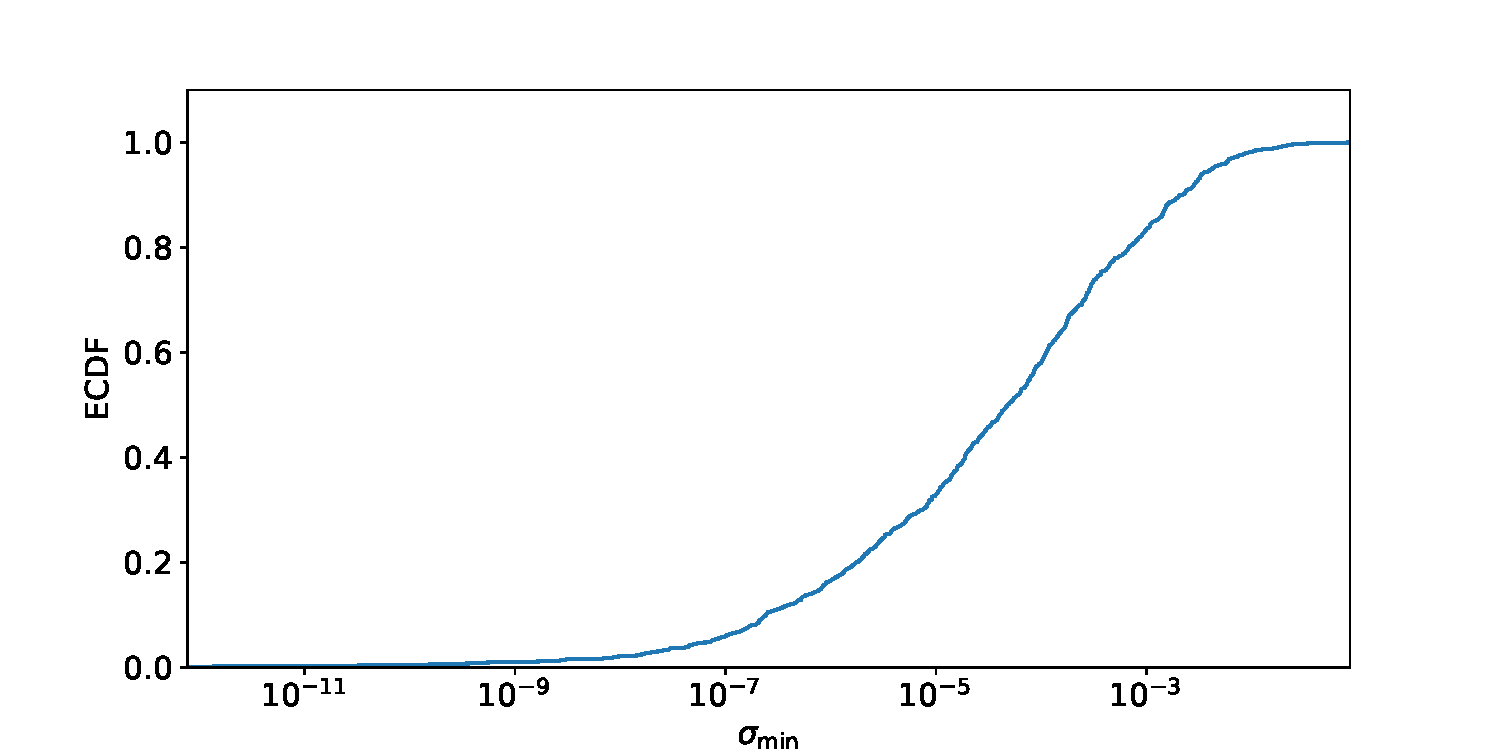
\includegraphics[width=\textwidth]{../2/triangular/ecdf/16.pdf}
  \caption{ECDF of the smallest singular values for all triangular matrices in
  the sample with $m=16$.}
  \label{fig:sigma_min_triangular_ECDF_16}
\end{figure}
\begin{figure}
  \centering
  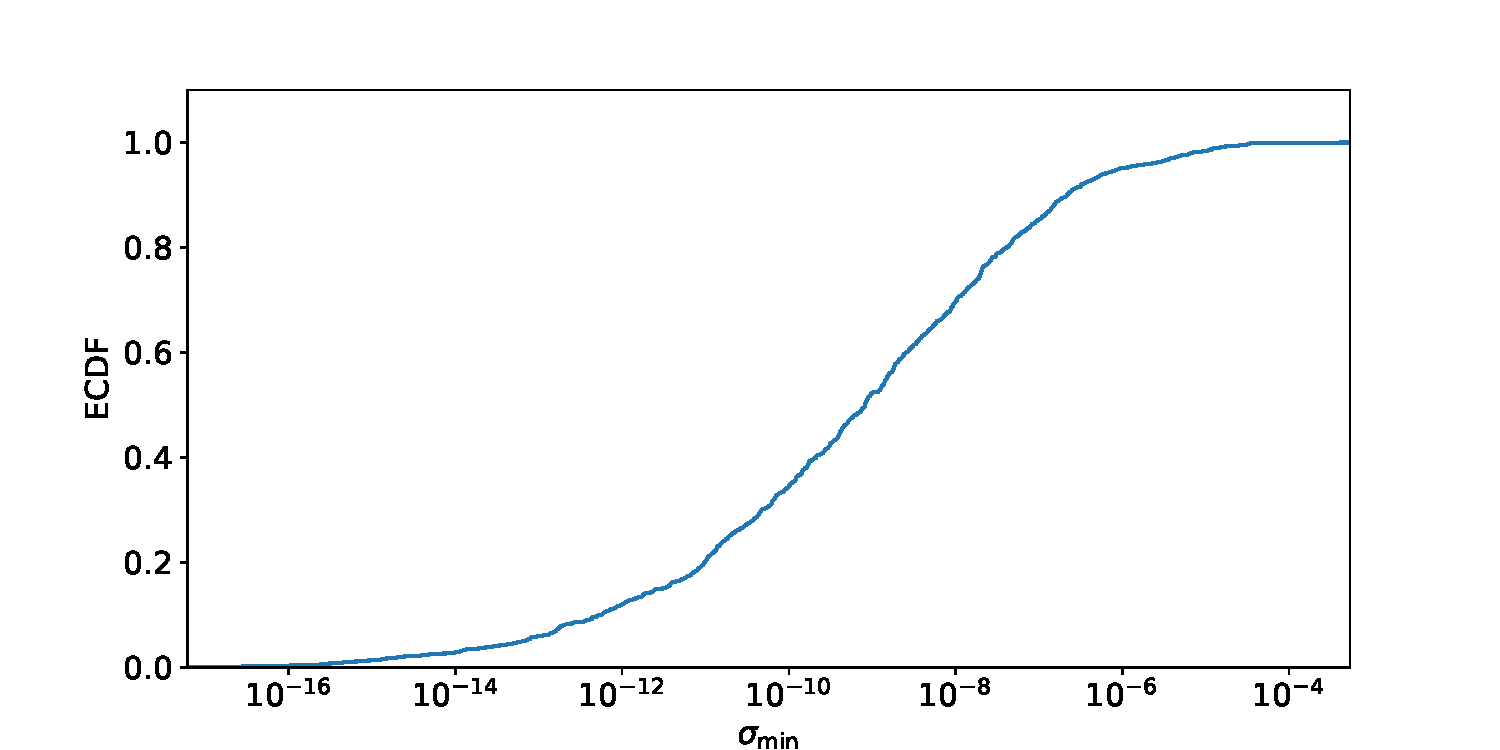
\includegraphics[width=\textwidth]{../2/triangular/ecdf/32.pdf}
  \caption{ECDF of the smallest singular values for all triangular matrices in
  the sample with $m=32$.}
  \label{fig:sigma_min_triangular_ECDF_32}
\end{figure}
\begin{figure}
  \centering
  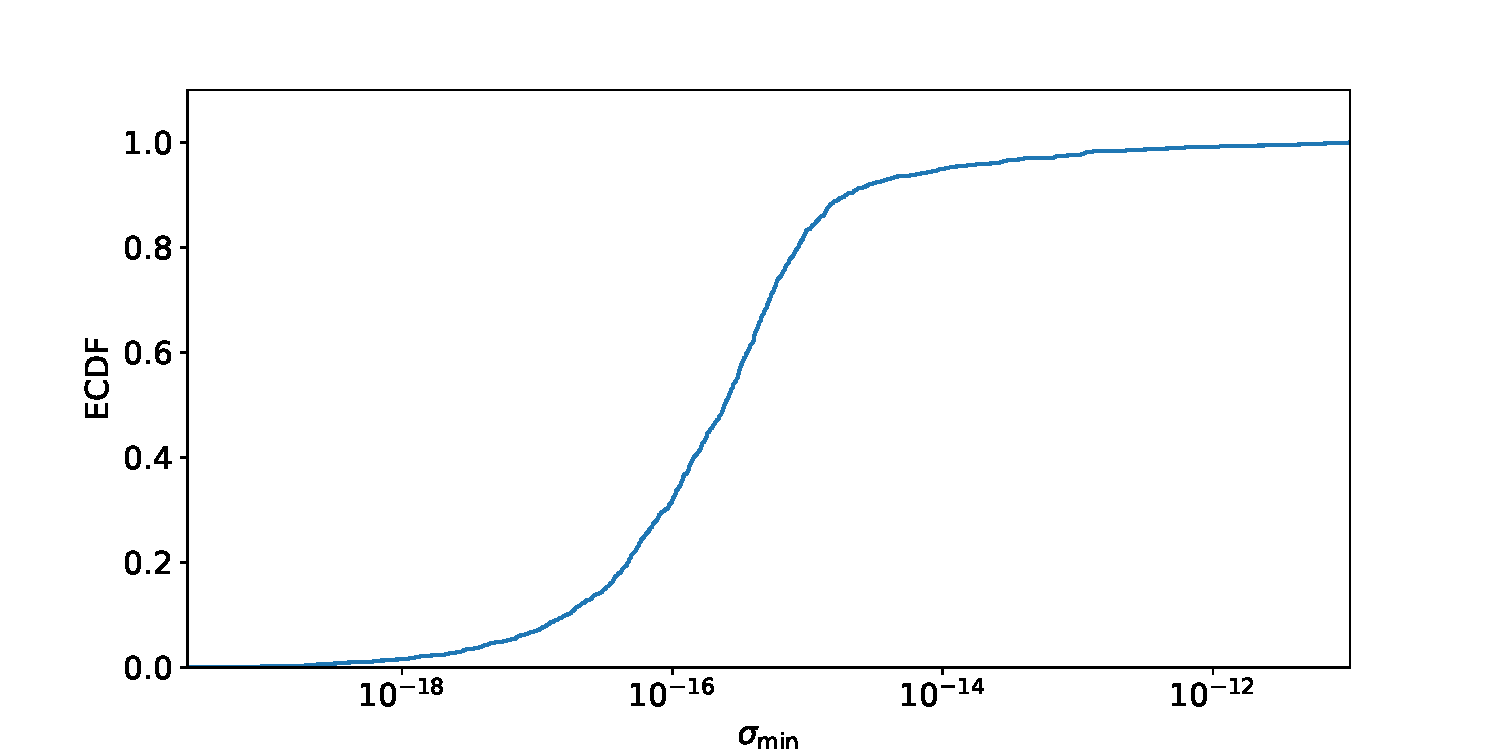
\includegraphics[width=\textwidth]{../2/triangular/ecdf/64.pdf}
  \caption{ECDF of the smallest singular values for all triangular matrices in
  the sample with $m=64$.}
  \label{fig:sigma_min_triangular_ECDF_64}
\end{figure}
\begin{figure}
  \centering
  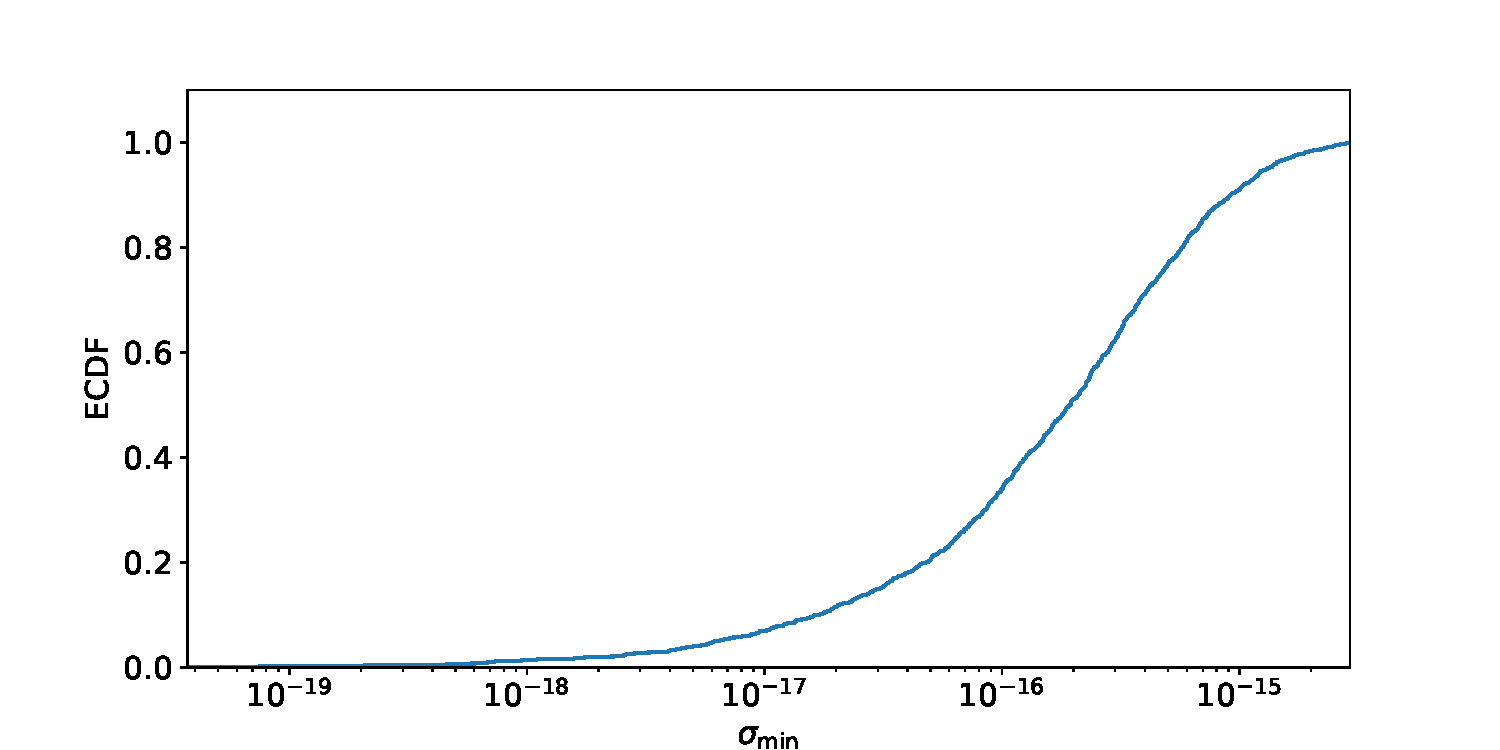
\includegraphics[width=\textwidth]{../2/triangular/ecdf/128.pdf}
  \caption{ECDF of the smallest singular values for all triangular matrices in
  the sample with $m=128$.}
  \label{fig:sigma_min_triangular_ECDF_128}
\end{figure}
\begin{figure}
  \centering
  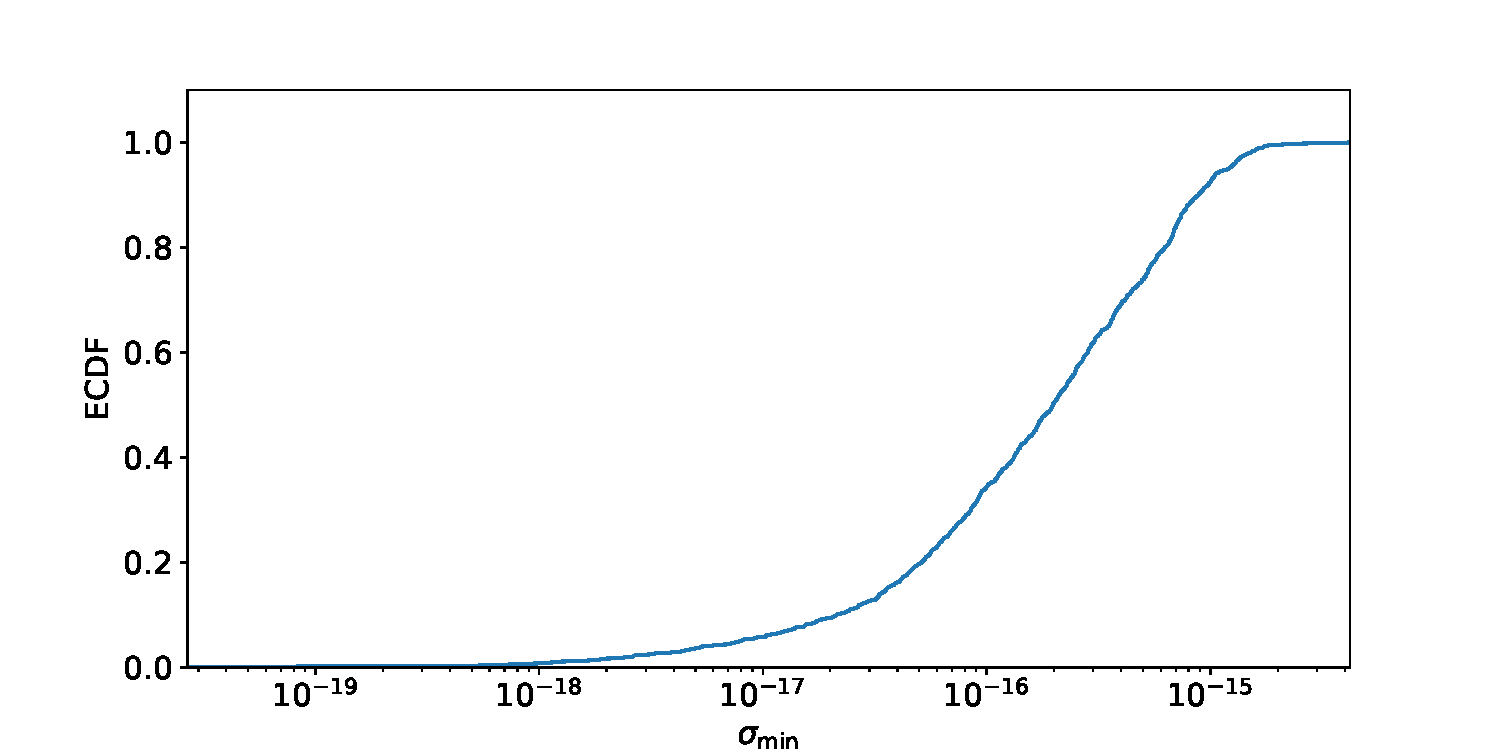
\includegraphics[width=\textwidth]{../2/triangular/ecdf/256.pdf}
  \caption{ECDF of the smallest singular values for all triangular matrices in
  the sample with $m=256$.}
  \label{fig:sigma_min_triangular_ECDF_256}
\end{figure}
\begin{figure}
  \centering
  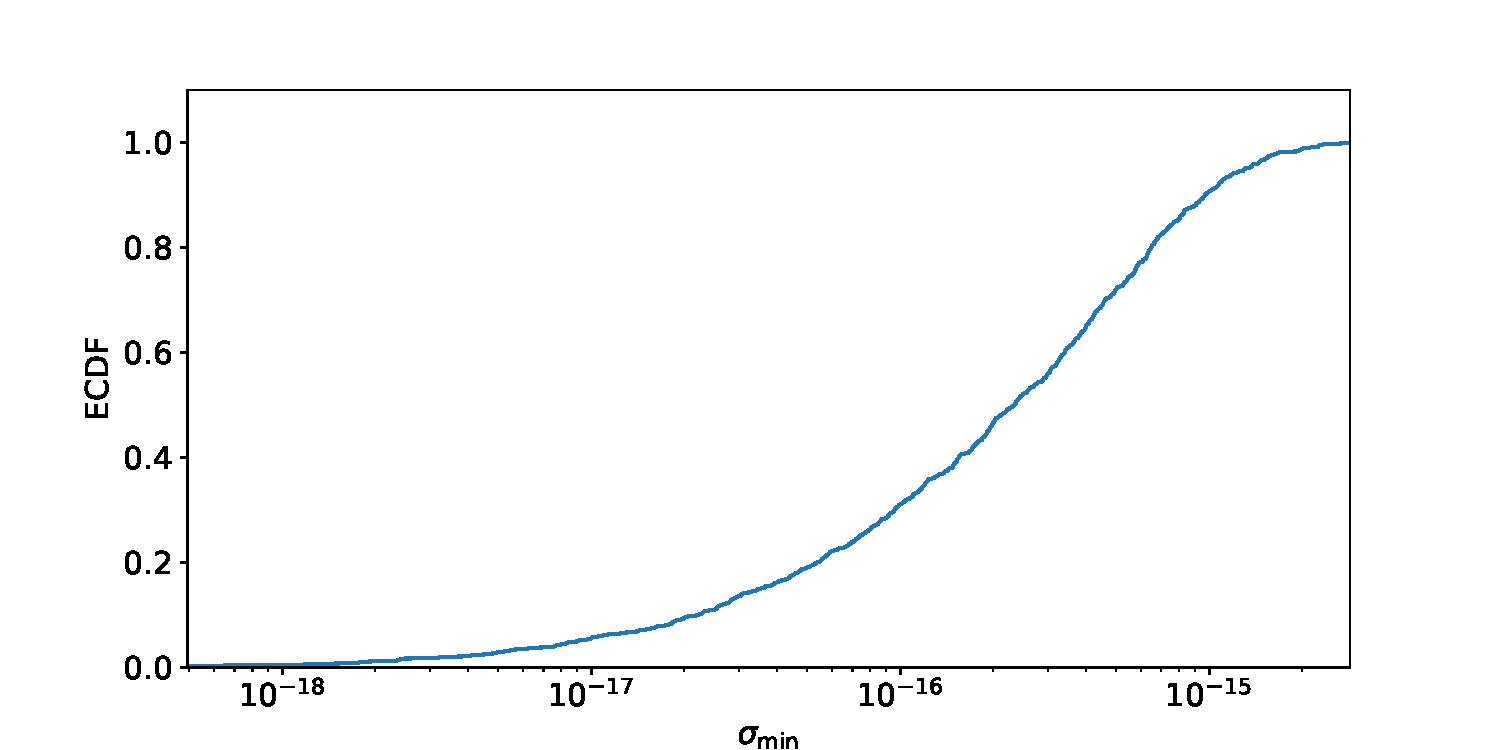
\includegraphics[width=\textwidth]{../2/triangular/ecdf/512.pdf}
  \caption{ECDF of the smallest singular values for all triangular matrices in
  the sample with $m=512$.}
  \label{fig:sigma_min_triangular_ECDF_512}
\end{figure}

\section*{3.}
\begin{figure}
  \centering
  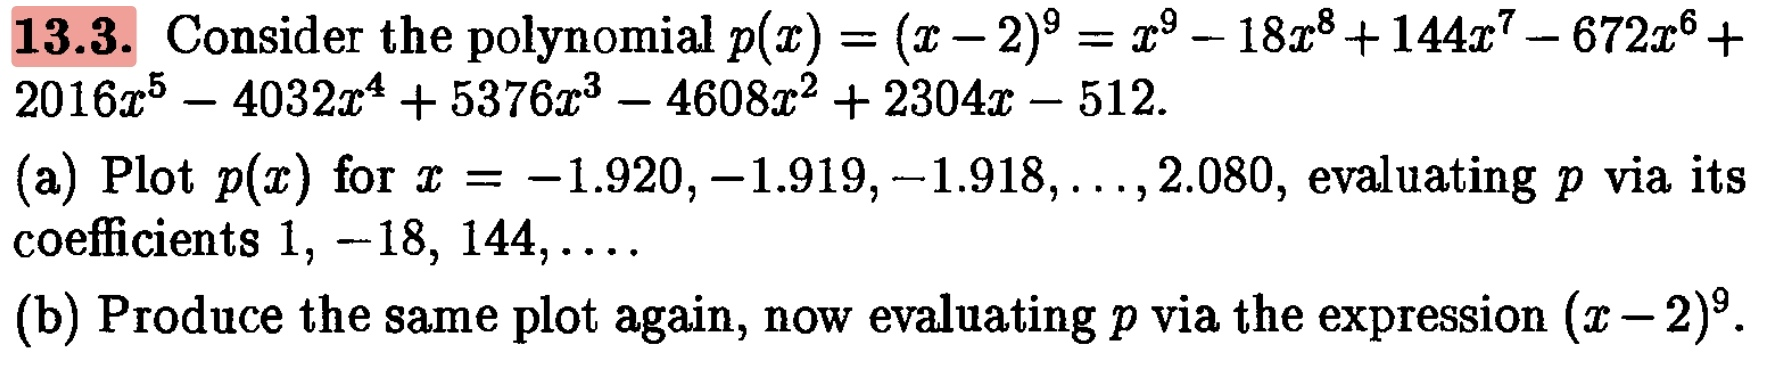
\includegraphics[width=\textwidth]{../3/13_3.jpg}
\end{figure}
Terrible assignment, probably due to the book being so old. I'll just do it and
it is worth full points, obviously not what the assignment is aiming for. It is
not saying what data types to use and it is also not asking for any discussion.
The assignment is literally just asking to create the two plots using the
different functions. Using any modern language the two plots will look exactly
the same. Obviously it is aiming at showing that the coefficient form will be
less accurate than the factorize form because of numerical instability for the
values close to zero. However, without using some ancient float data type
and/or a terrible language/library, that's simply not the case anymore today.
\textit{Numpy} handles such scenarios with ease (I would assume primarily
because of proper use of guard digits, but I don't really know the details of
\textit{Numpy}'s implementation), even when using single precision floats
(which I did even though the assignment does not ask for it). To actually see a
difference one has to use half precision, however in that case we actually get
overflows and the range that is asked for by the assignment can't even be
represented. So here you go, two identical plots in Figure~\ref{fig:3_a} and
Figure~\ref{fig:3_b} \quad :D

\FloatBarrier
\subsection*{(a)}
\begin{figure}
  \centering
  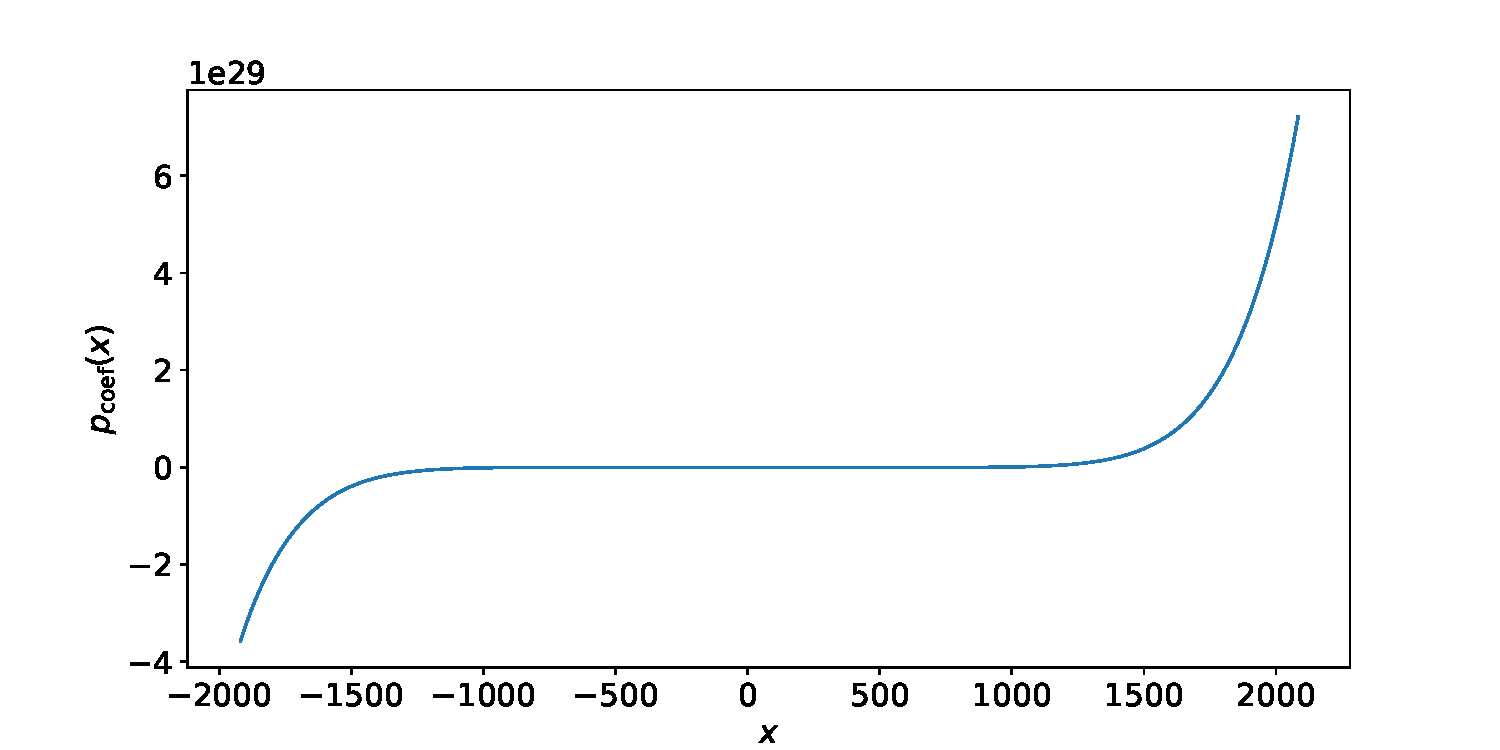
\includegraphics[width=\textwidth]{../3/a.pdf}
  \caption{Plot of the polynomial using the coefficient form for evaluation and
  single precision floating point numbers.}
  \label{fig:3_a}
\end{figure}

\FloatBarrier
\subsection*{(b)}
\begin{figure}
  \centering
  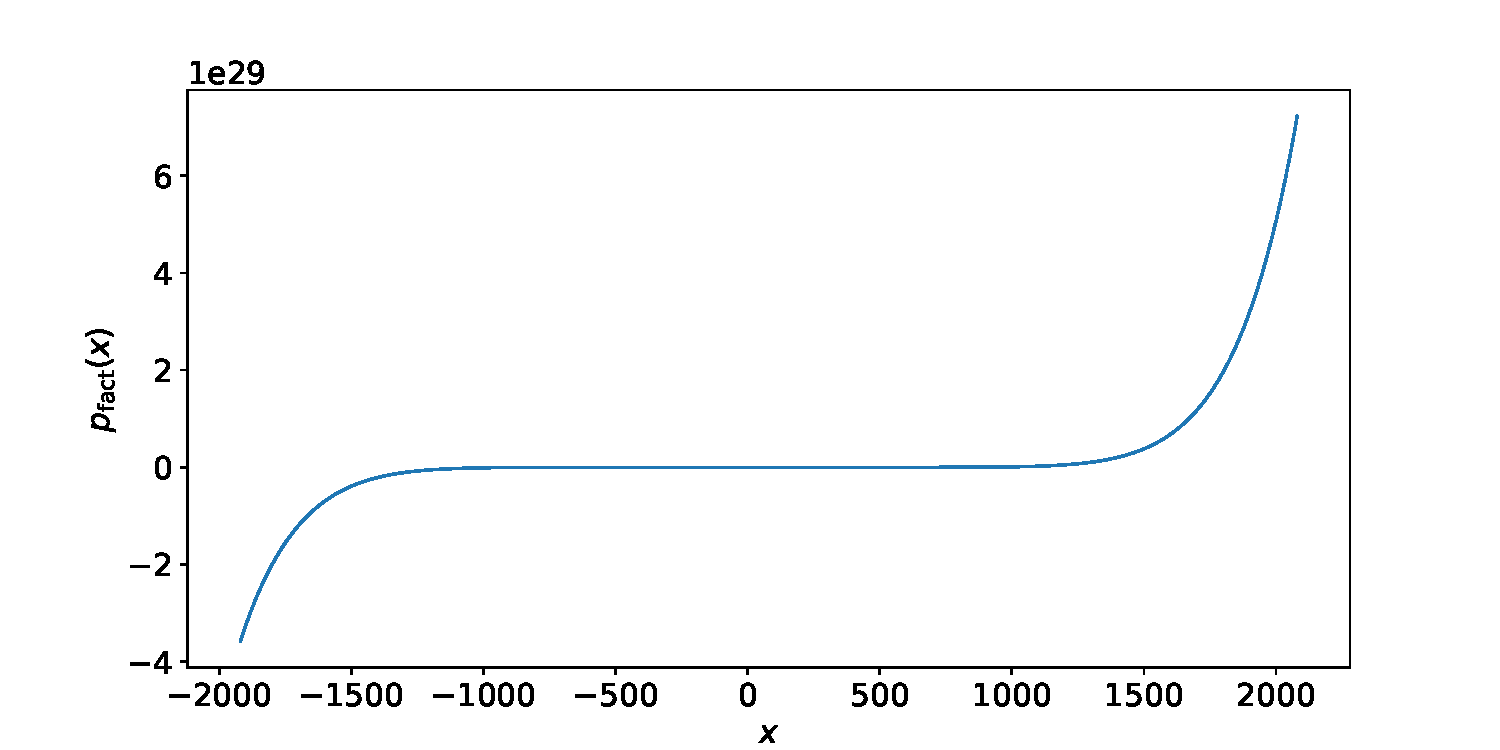
\includegraphics[width=\textwidth]{../3/b.pdf}
  \caption{Plot of the polynomial using the factorized form for evaluation and
  single precision floating point numbers.}
  \label{fig:3_b}
\end{figure}
For good measure (even though this terribly designed assignment does not ask
for it) I include a plot showing the difference between the two forms using
single precision in Figure~\ref{fig:3_a_b_difference}. We can see the usual
pattern arising due to numerical instability when subtracting equally large
numbers. However, the range where the polynomial is zero is totally fine, even
when subtracting the two representations which are both numerically zero from
each other. Trivial scenarios like this are simply not an issue any more for
any modern computing system.
\begin{figure}[H]
  \centering
  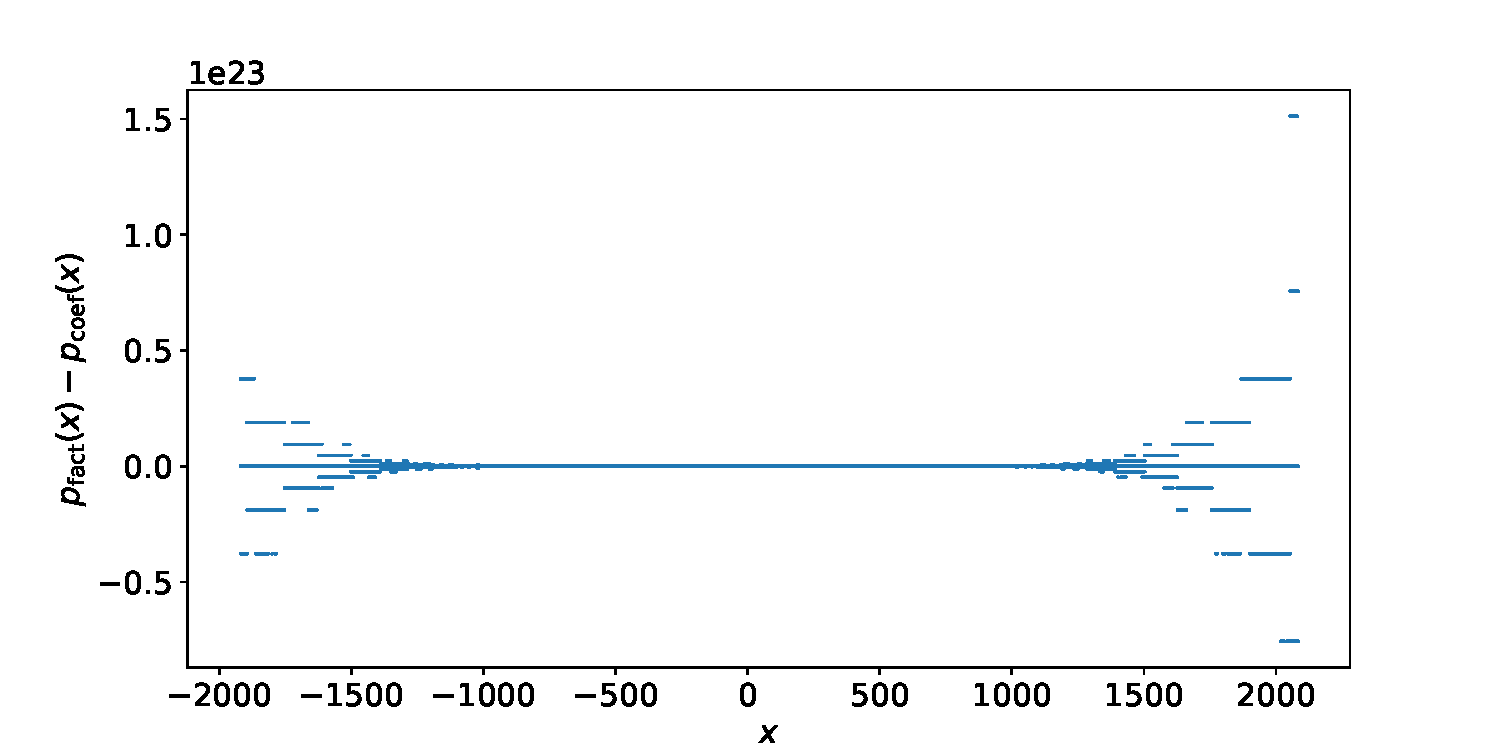
\includegraphics[width=\textwidth]{../3/a_b_diff.pdf}
  \caption{Difference between the coefficient and factorized form of the
  polynomial using single precision.}
  \label{fig:3_a_b_difference}
\end{figure}

\FloatBarrier
\section*{4.}
\textbf{None of this has been taught in class in time to finish the
assignment!}
See the following handwritten pages.
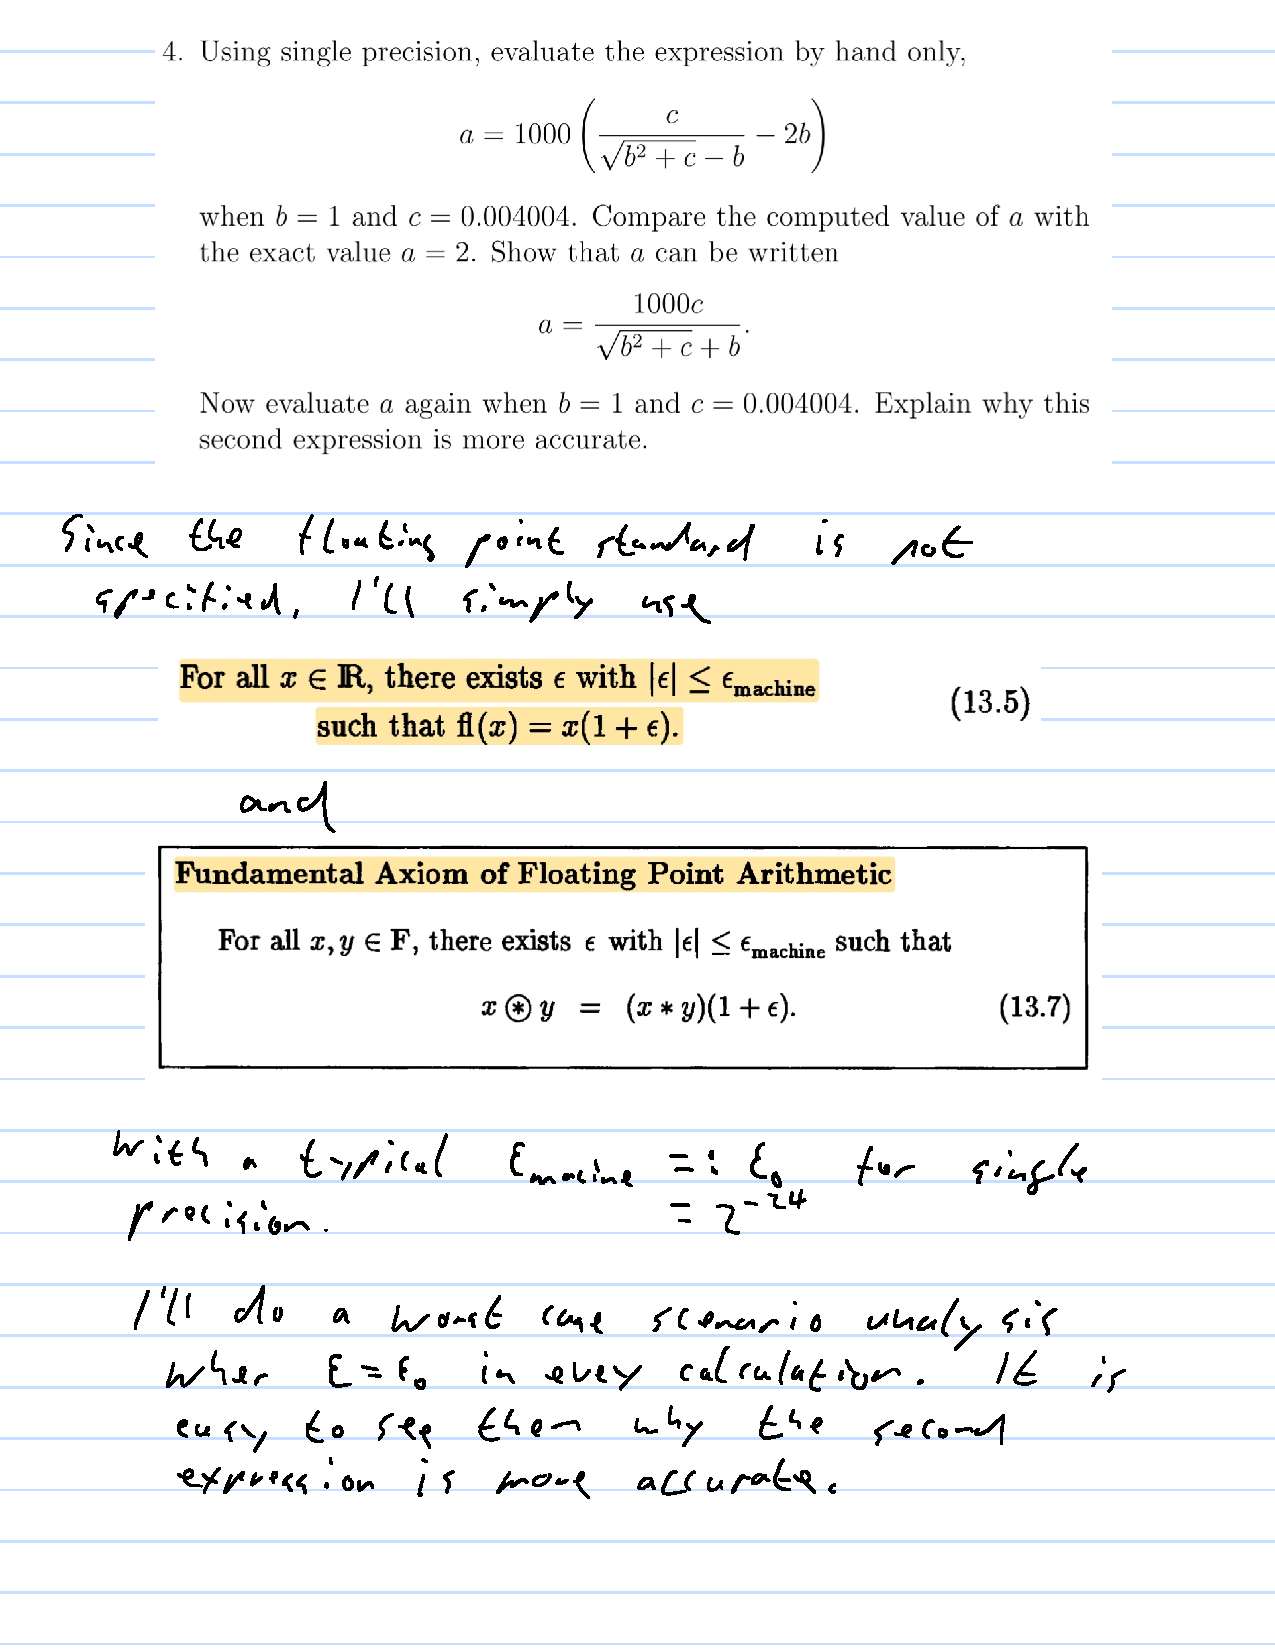
\includepdf{../4/4_1.pdf}
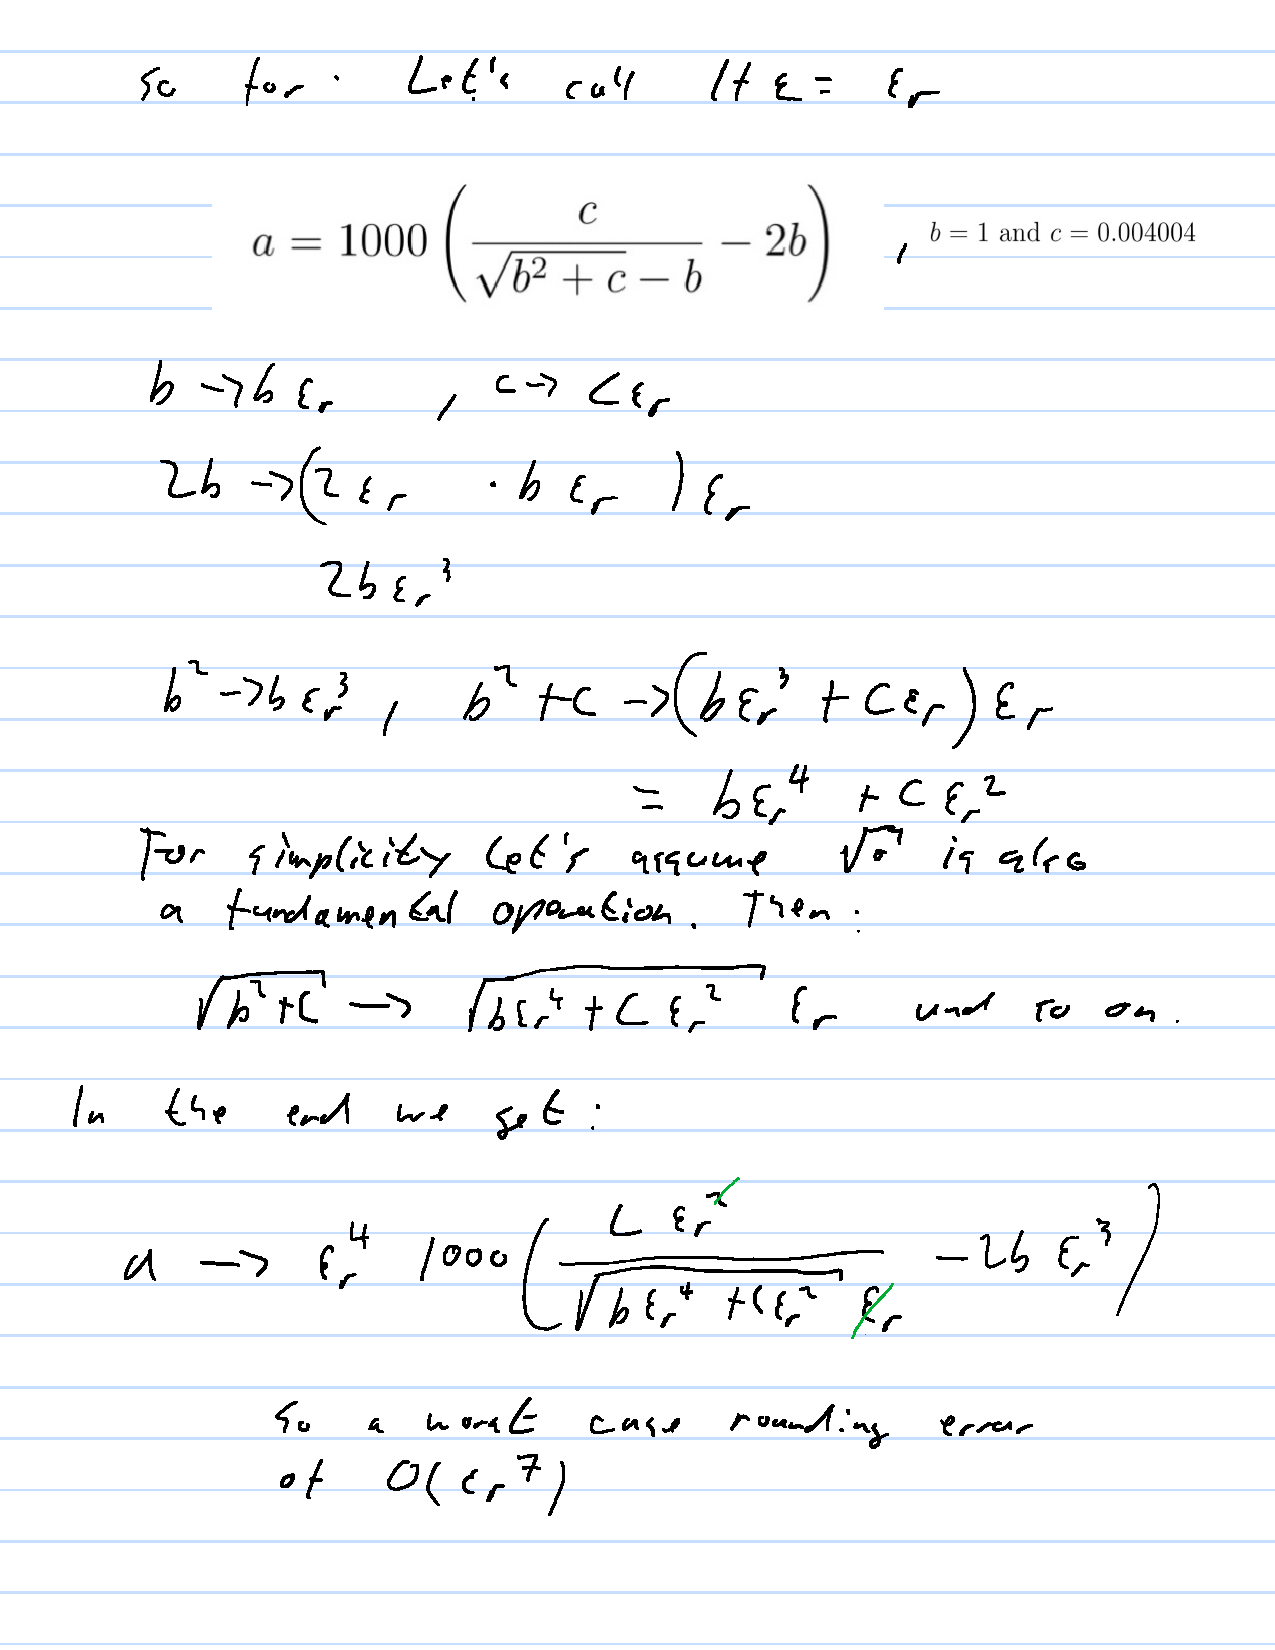
\includepdf{../4/4_2.pdf}
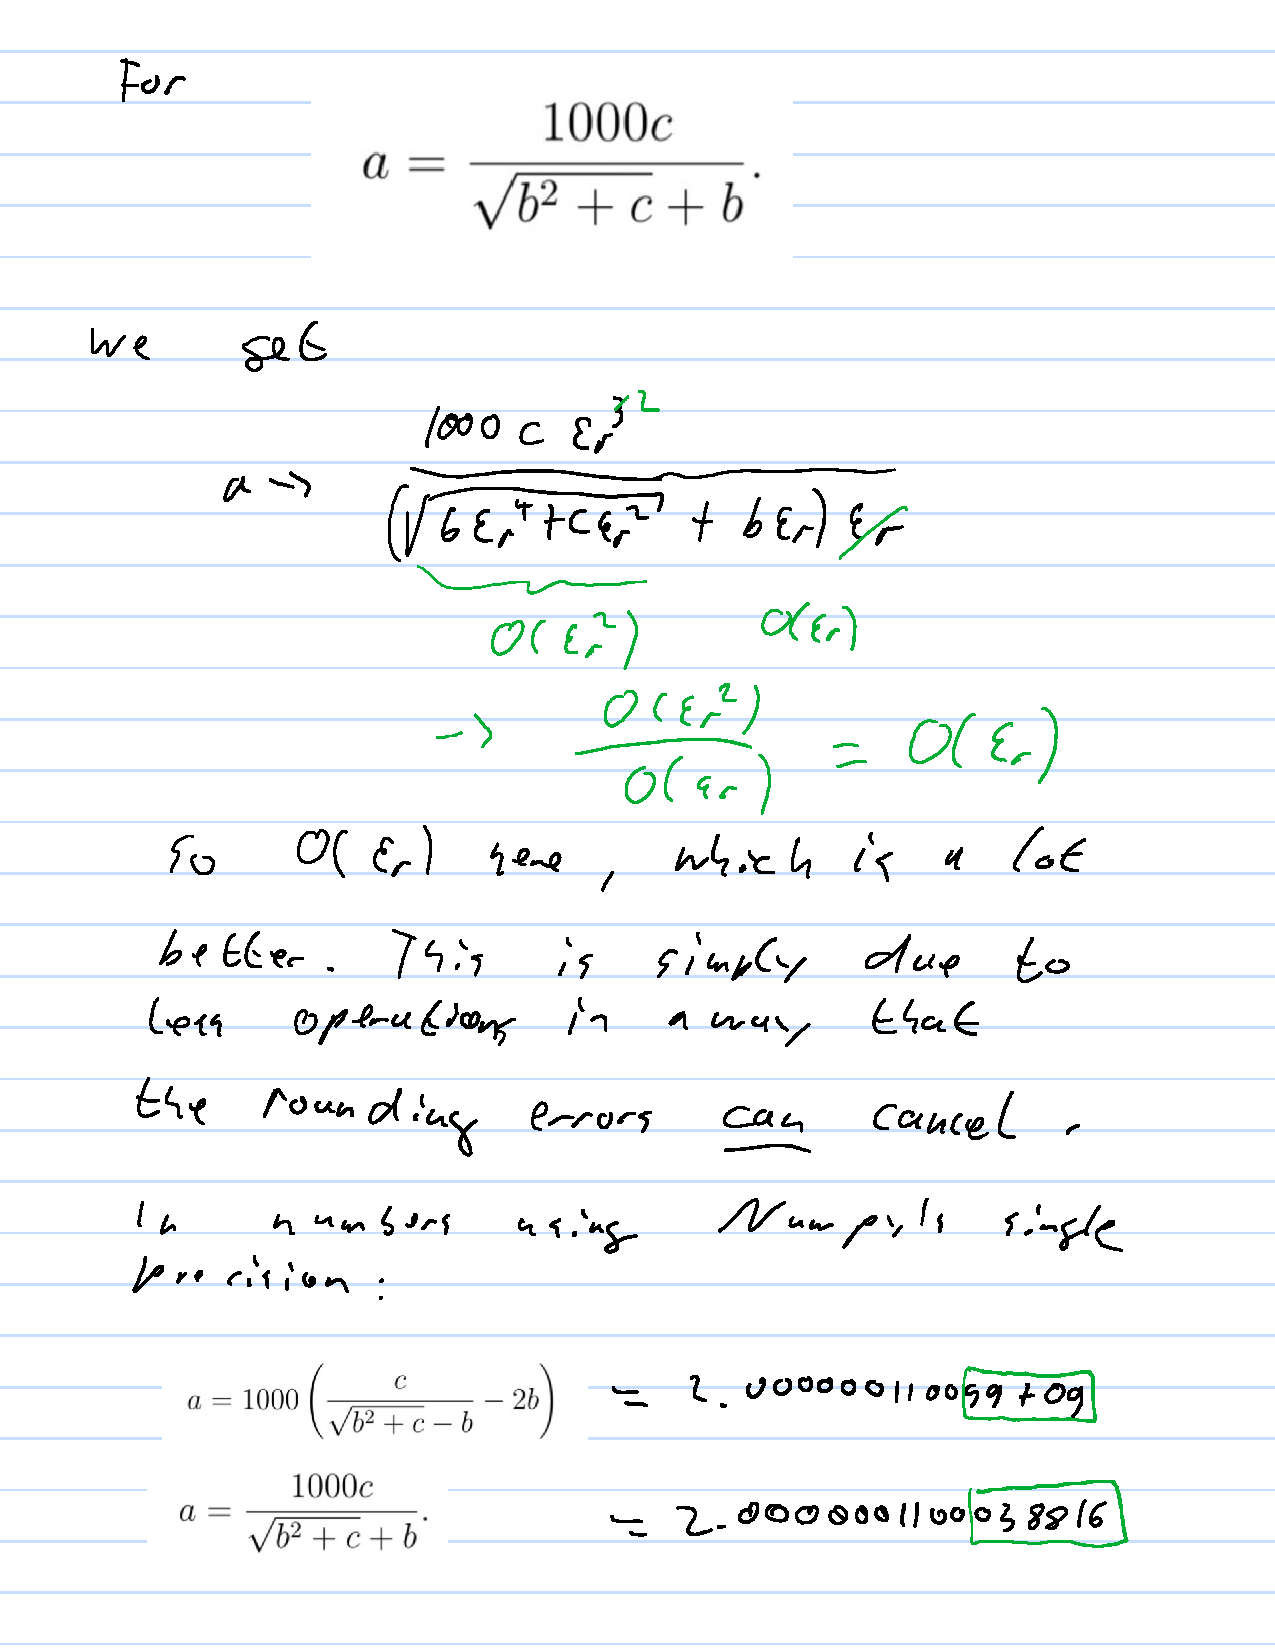
\includepdf{../4/4_3.pdf}
\end{document}
